\documentclass[mathpazo]{cicp}

% 基础数学支持包
\usepackage{times,amsmath,amsbsy,amssymb,amscd,mathrsfs}
\usepackage{mathtools}
%\usepackage{algorithm2e} 

% 表格和布局支持
\usepackage{multicol,multirow}
\usepackage{booktabs}

% 图形和绘图支持 - 保留核心功能
\usepackage[labelformat=empty]{subfig}
\usepackage{tikz,tikz-cd}
\usepackage{pgfplots}
\pgfplotsset{compat=newest}
\pgfplotsset{plot coordinates/math parser=false}
\newlength\fwidth

% 颜色和超链接
\definecolor{myBlue}{rgb}{0.0,0.0,0.55}
\usepackage[pdftex,colorlinks=true,citecolor=myBlue,linkcolor=myBlue]{hyperref}

% 保留用户实际使用的命令
\newcommand{\LC}[1]{\textcolor{red!80!black}{#1}}
\newcommand{\XH}[1]{\textcolor{cyan}{#1}}
\newcommand{\CC}[1]{\textcolor{orange}{#1}}

\usepackage{enumerate,xspace}

% 重要数学命令
\newcommand{\dx}{\,{\rm d}x}
\newcommand{\dd}{\,{\rm d}}
\newcommand{\deq}{\stackrel{\rm def}{=}}
\newcommand{\mbb}{\mathbb}
\newcommand{\mbf}{\bs}
\newcommand{\bs}{\boldsymbol}
\newcommand{\mcal}{\mathcal}
\newcommand{\lla}{\langle}
\newcommand{\rra}{\rangle}
\newcommand{\supp}{\operatorname{supp}}
\newcommand{\range}{\operatorname{range}}

\DeclarePairedDelimiter\ceil{\lceil}{\rceil}
\DeclarePairedDelimiter\floor{\lfloor}{\rfloor}

% 颜色命令
\newcommand{\red}{\color{red}}
\newcommand{\green}{\color{green}}
\newcommand{\blue}{\color{blue}}
\newcommand{\gray}{\color{gray}}

% 数学运算符
\DeclareMathOperator*{\img}{img}
\DeclareMathOperator*{\spa}{span}
\DeclareMathOperator*{\diag}{diag}
\newcommand{\curl}{{\rm curl\,}}
\renewcommand{\div}{\operatorname{div}}
\newcommand{\grad}{{\rm grad\,}}
\DeclareMathOperator*{\rot}{rot}
\DeclareMathOperator*{\var}{Var}
\DeclareMathOperator{\rank}{rank}
\DeclareMathOperator{\dist}{dist}
\newcommand{\tr}{\operatorname{tr}}
\newcommand{\dev}{\operatorname{dev}}
\newcommand{\sym}{\operatorname{sym}}
\newcommand{\skw}{\operatorname{skw}}
\newcommand{\spn}{\operatorname{spn}}
\newcommand{\defm}{\operatorname{def}}
\newcommand{\hess}{\operatorname{hess}}

% 常用的数学符号
\newcommand{\norm}[1]{\left\Vert#1\right\Vert}
\newcommand{\snorm}[1]{\left\vert#1\right\vert}
\newcommand{\vertiii}[1]{{\left\vert\kern-0.25ex\left\vert\kern-0.25ex\left\vert #1 \right\vert\kern-0.25ex\right\vert\kern-0.25ex\right\vert}}



%\usepackage{times,amsmath,amsbsy,amssymb,amscd,mathrsfs}
%%\usepackage{slashbox}\usepackage{graphicx,subfigure,epstopdf,wrapfig,chemarrow}
%
%\usepackage{algorithm2e} 
%\usepackage{multicol,multirow}
%\usepackage{mathtools}
%\usepackage[usenames,dvipsnames,svgnames,table]{xcolor}
%\usepackage[all]{xy}
%\usepackage{wrapfig}
%\usepackage{tcolorbox}
%\usepackage{booktabs} 
%
%\usepackage[labelformat=empty]{subfig}
%%\usepackage[hang,small,bf]{caption}
%
%\usepackage{tikz,tikz-cd}
%\usepackage[utf8]{inputenc}
%\usepackage{pgfplots} 
%\usepackage{pgfgantt}
%\usepackage{pdflscape}
%\pgfplotsset{compat=newest} 
%\pgfplotsset{plot coordinates/math parser=false}
%\newlength\fwidth
%
%%\usepackage[notcite,notref]{showkeys}
%\usepackage[numbered]{mcode}
%
%\definecolor{myBlue}{rgb}{0.0,0.0,0.55}
%%\definecolor{green}{rgb}{0.0,0.7,0.2}
%\usepackage[pdftex,colorlinks=true,citecolor=myBlue,linkcolor=myBlue]{hyperref}
%
%\usepackage[hyperpageref]{backref}
%
%%\newcommand{\LC}[1]{\textcolor{cyan}{#1}}
%\newcommand{\LC}[1]{\textcolor{red!80!black}{#1}}
%\newcommand{\XH}[1]{\textcolor{cyan}{#1}}
%\newcommand{\CC}[1]{\textcolor{orange}{#1}}
%
%\usepackage{comment,enumerate,multicol,xspace}
%
%  \newcounter{mnote}
%  \setcounter{mnote}{0}
%  \newcommand{\mnote}[1]{\addtocounter{mnote}{1}
%    \ensuremath{{}^{\bullet\arabic{mnote}}}
%    \marginpar{\footnotesize\em\color{red}\ensuremath{\bullet\arabic{mnote}}#1}}
%  \let\oldmarginpar\marginpar
%    \renewcommand\marginpar[1]{\-\oldmarginpar[\raggedleft\footnotesize #1]%
%    {\raggedright\footnotesize #1}}
%
%%\usepackage[pdftex,dvipsnames]{xcolor}
%
%%\usepackage{xargs} % Use more than one optional parameter in a new commands
%%\usepackage[colorinlistoftodos,prependcaption,textsize=footnotesize]{todonotes}
%%
%%\newcounter{mycomment}
%%\newcommand{\mycomment}[2][]{%
%%% initials of the author (optional) + note in the margin
%%\refstepcounter{mycomment}%
%%{%
%%\todo[linecolor=blue,backgroundcolor=blue!25,bordercolor=blue]{%
%%\textbf{Comment [{\sc #1\themycomment}]:}\\#2}%
%%}}
%%
%%\newcommandx{\change}[2][1=]
%%{\todo[linecolor=OliveGreen,backgroundcolor=OliveGreen!25,bordercolor=OliveGreen,#1]{%
%%{\sc Change}:\\#2}}
%%
%%\newcommandx{\improvement}[2][1=]
%%{\todo[linecolor=Plum,backgroundcolor=Plum!25,bordercolor=Plum,#1]{%
%%{\sc Improvement}:\\#2}}
%%
%%\newcommandx{\unsure}[2][1=]
%%{\todo[linecolor=red,backgroundcolor=red!25,bordercolor=red,#1]{%
%%{\sc Unsure}:\\ #2}}
%%
%
%% \newcommand{\mnote}[1]{}
%\newcommand{\breakline}{
%\begin{center}
%------------------------------------------------------------------------------------------------------------
%\end{center}
%}
%%\usepackage{geometry}
%%%\usepackage{graphicx,pst-eps,epstopdf}
%%\geometry{letterpaper, margin=1.5in}
%
%%\newtheorem{theorem}{Theorem}[section]
%%\newtheorem{lemma}[theorem]{Lemma}
%\newtheorem{corollary}[theorem]{Corollary}
%%\newtheorem{proposition}[theorem]{Proposition}
%%\newtheorem{definition}[theorem]{Definition}
%%\newtheorem{example}[theorem]{Example}
%\newtheorem{exercise}[theorem]{Exercise}
%\newtheorem{question}[theorem]{Question}
%%\newtheorem{remark}[theorem]{Remark}
%\newtheorem{alg}[theorem]{Algorithm}
%%\newtheorem{answer}[proof]{Question}
%
%\newcommand{\dx}{\,{\rm d}x}
%\newcommand{\dd}{\,{\rm d}}
%\newcommand{\deq}{\stackrel{\rm def}{=}}
%\newcommand{\mbb}{\mathbb}
%\newcommand{\mbf}{\bs}
%\newcommand{\bs}{\boldsymbol}
%\newcommand{\mcal}{\mathcal}
%\newcommand{\mc}{\mcode}
%\newcommand{\lla}{\langle}
%\newcommand{\rra}{\rangle}
%\newcommand{\supp}{\operatorname{supp}}
%\newcommand{\range}{\operatorname{range}}
%\newcommand{\PartSize}{\fontsize{0.85cm}{0.85cm}\selectfont} 
%\newcommand{\mscr}{\mathscr}
%\DeclarePairedDelimiter\ceil{\lceil}{\rceil}
%\DeclarePairedDelimiter\floor{\lfloor}{\rfloor}
%
%%\newcommand{\span}{\rm span}
%\newcommand{\red}{\color{red}}
%\newcommand{\green}{\color{green}}
%\newcommand{\blue}{\color{blue}}
%\newcommand{\gray}{\color{gray}}
%
%%\DeclareMathOperator*{\curl}{curl}
%\DeclareMathOperator*{\img}{img}
%\DeclareMathOperator*{\spa}{span}
%\DeclareMathOperator*{\diag}{diag}
%\newcommand{\curl}{{\rm curl\,}}
%\renewcommand{\div}{\operatorname{div}}
%%\renewcommand{\grad}{\operatorname{grad}}
%\newcommand{\grad}{{\rm grad\,}}
%%\DeclareMathOperator*{\tr}{tr}
%\DeclareMathOperator*{\rot}{rot}
%\DeclareMathOperator*{\var}{Var}
%\DeclareMathOperator{\rank}{rank}
%\DeclareMathOperator{\dist}{dist}
%%\DeclareMathOperator{\span}{span}
%\newcommand{\tr}{\operatorname{tr}}
%\newcommand{\dev}{\operatorname{dev}}
%\newcommand{\sym}{\operatorname{sym}}
%\newcommand{\skw}{\operatorname{skw}}
%\newcommand{\spn}{\operatorname{spn}}
%\newcommand{\mspn}{\operatorname{mspn}}
%\newcommand{\vspn}{\operatorname{vspn}}
%\newcommand{\mskw}{\operatorname{mskw}}
%\newcommand{\vskw}{\operatorname{vskw}}
%\newcommand{\defm}{\operatorname{def}}
%\newcommand{\hess}{\operatorname{hess}}
%\newcommand{\inc}{\operatorname{inc}}
%\newcommand{\dex}{\operatorname{dex}}
%
%\newcommand{\step}[1]{\noindent\raisebox{1.5pt}[10pt][0pt]{\tiny\framebox{$#1$}}\xspace}
%
%%\usepackage[margins]{trackchanges}
%%\renewcommand{\initialsOne}{chen}
%
%\newcommand{\norm}[1]{\left\Vert#1\right\Vert}
%\newcommand{\snorm}[1]{\left\vert#1\right\vert}
%\newcommand{\vertiii}[1]{{\left\vert\kern-0.25ex\left\vert\kern-0.25ex\left\vert #1 
%    \right\vert\kern-0.25ex\right\vert\kern-0.25ex\right\vert}}


\let\listofalgorithms\relax
\let\listalgorithmname\relax
\usepackage{algorithm}
\usepackage{algpseudocode}
\usepackage{stmaryrd}
\usepackage{scalefnt}
\usepackage{graphicx}
\usepackage{caption}
\usepackage{subcaption}
\usepackage{booktabs}
\usepackage{multirow}
\usepackage{multicol}
\usepackage{float}
\usepackage{bm}

% Float placement: discourage float pages for half-page figures
\renewcommand{\topfraction}{0.85}
\renewcommand{\bottomfraction}{0.5}
\renewcommand{\textfraction}{0.1}
\renewcommand{\floatpagefraction}{0.75}

\renewcommand{\thealgorithm}{\arabic{section}.\arabic{algorithm}}
\renewcommand{\algorithmicrequire}{\textbf{Input:}}
\renewcommand{\algorithmicensure}{\textbf{Output:}}

\captionsetup[figure]{font=rm}

\begin{document}
\title[Arbitrary-Order Hu--Zhang Elements for Topology Optimization]{Arbitrary-Order Hu--Zhang Mixed Finite Element Methods for Density-Based Topology Optimization}

\author[He L, Chen C Y, Wei H Y]{Liang He\affil{1}, Chunyu Chen\affil{2}, Huayi Wei\affil{3}}
\address{
\affilnum{1}\ 
School of Mechanics and Aerospace Engineering, Dalian University of Technology, Dalian 116024, China\\
\affilnum{2}\ 
School of Mathematical Sciences, Peking University, Beijing 100871, China\\
\affilnum{3}\ 
School of Mathematics and Computational Science, Xiangtan University; 
National Center of Applied Mathematics in Hunan, Hunan Key Laboratory for 
Computation and Simulation in Science and Engineering, Xiangtan 411105, China
}

\emails{
	{\tt heliang@dlut.edu.cn} (L.~He),
	{\tt cbtxs@math.pku.edu.cn} (C.~Chen),
	{\tt weihuayi@xtu.edu.cn} (H.~Wei)
}

\begin{abstract}
In density-based topology optimization, displacement-based finite elements recover stresses from displacement gradients but generally do not guarantee inter-element traction continuity. Low-order displacement elements are prone to volumetric locking in nearly incompressible regimes. To address these issues, this paper develops an arbitrary-order Hu--Zhang mixed finite element framework for density-based topology optimization on simplicial meshes. The framework treats symmetric stress and displacement as independent unknowns. Combining jump stabilization for lower polynomial orders with local corner relaxation, we formulate two optimization models: compliance minimization and volume minimization subject to local stress constraints. We derive consistent adjoint sensitivities that account for the design dependence of the right-hand side introduced by traction lifting. The proposed topology optimization framework is implemented in FEALPy. Two-dimensional numerical examples show that both native higher-order and low-order stabilized formulations exhibit convergence, and the unified optimization workflow is applicable across all investigated discrete polynomial degrees. In standard compliance optimization, the mixed and displacement-based methods yield comparable topologies and compliance values. Mesh convergence results for the fully solid bearing domain show that Hu--Zhang elements exhibit similar compliance convergence trends under compressible and nearly incompressible conditions, without the pronounced loss of accuracy observed for linear displacement elements. In nearly incompressible topology optimization, Hu--Zhang elements effectively mitigate the effects of volumetric locking on the optimization results. The resulting designs are comparable to those obtained with quadratic displacement elements in both topology and compliance evaluated using a common discretization. Local stress constraints are evaluated directly from the primary stress variables without stress recovery, with the discrete stress naturally preserving inter-element normal traction continuity.
\end{abstract}

\ams{65N30, 74S05, 74P05, 74B05}
\keywords{Hu--Zhang mixed finite elements, arbitrary-order approximation, density-based topology optimization, nearly incompressible elasticity, local stress constraints}

\maketitle
% Display author emails without designating a corresponding author.
\begingroup
\renewcommand{\thefootnote}{}
\makeatletter
\footnotetext{\@setemails}
\makeatother
\endgroup

\section{Introduction}
\label{sec:introduction}

Topology optimization (TO) provides a systematic numerical design tool for high-performance lightweight structures by optimizing the spatial distribution of material within a prescribed design domain. Since the continuum material distribution approach was introduced by Bends{\o}e~\cite{Bendsoe1989}, density-based topology optimization, particularly represented by the Solid Isotropic Material with Penalization (SIMP) method, has been widely adopted due to its conceptual clarity, algorithmic maturity, and broad engineering applicability~\cite{BendsoeSigmund2003}. In classical implementations, the linear elastic state equations are predominantly discretized using standard conforming displacement-based Lagrange finite element methods (LFEM), where stress tensors are subsequently recovered within element interiors via numerical gradients of the discrete displacement fields. While such a displacement-driven paradigm is computationally efficient and sufficient for conventional compliance minimization problems, it encounters severe discretization errors and numerical bottlenecks in design problems governed by accurate local stress evaluation or nearly incompressible material behavior.

In local stress-constrained problems, constraints are imposed element-wise, whose quantity scales with the mesh size, and their values are strictly dictated by the accuracy of the discrete stress field. In standard displacement elements, differentiating displacement shape functions reduces the stress approximation accuracy by one order (e.g., linear elements yield only piecewise constant stresses), accompanied by non-physical discontinuous jumps in both normal and tangential stresses across element interfaces. If these post-processed discrete stresses are directly substituted into local constraints, the mutual coupling among discretization errors, smoothing strategies, and the optimization model readily induces local stress oscillations or traps the structural evolution in over-optimized designs~\cite{Duysinx1998,Le2010,Paris2010,daSilva2019}. In nearly incompressible material regimes, as Poisson's ratio approaches the incompressible limit ($\nu_0 \to 0.5$), the bulk modulus of plane-strain or three-dimensional continua tends to infinity relative to the shear modulus, imposing a stringent divergence-free deformation constraint ($\operatorname{div}\boldsymbol{u} \approx 0$). Owing to the lack of sufficient deformation degrees of freedom in the discrete displacement space, standard low-order displacement elements suffer from severe volumetric locking~\cite{Puso2006}, which artificially exaggerates structural stiffness and produces pathological thin members and spurious hinges during topological evolution~\cite{SigmundClausen1998,Kumar2017}.

Mixed finite element methods offer an intrinsic variational pathway to overcome the aforementioned mechanical challenges~\cite{BoffiBrezziFortin2013}. Based on the Hellinger--Reissner two-field variational principle, the symmetric stress $\boldsymbol{\sigma}$ and displacement $\boldsymbol{u}$ are treated simultaneously as independent unknowns. The stress trial functions belong directly to the symmetric tensor $H(\operatorname{div})$ space, naturally guaranteeing strict continuity of normal tractions across inter-element boundaries, while the divergence equilibrium equation is satisfied exactly in the weak form. Because the compliance bilinear form remains uniformly bounded in the incompressible limit, mixed elements satisfying the discrete inf-sup (Babu\v{s}ka--Brezzi) condition fundamentally circumvent volumetric locking~\cite{Stenberg1986,BrezziAdams2003}. The truly-mixed topology optimization studies by Bruggi and Venini~\cite{BruggiVenini2007,BruggiVenini2008} and Bruggi~\cite{Bruggi2016} demonstrated that directly discretizing stress and displacement provides an effective means for nearly incompressible structural design and stress-constrained optimization. However, most existing mixed finite element topology optimization literature is restricted to lowest-order discretizations, structured quadrilateral meshes, or specific hybridized formulations. For unstructured simplicial meshes (triangles and tetrahedra), constructing strictly symmetric and conforming $H(\operatorname{div})$ spaces has long posed substantial mathematical difficulties, often necessitating additional multipliers to relax the symmetry into weakly symmetric formulations~\cite{ArnoldWinther2002,AdamsCockburn2005,Arnold2007}.

The Hu--Zhang mixed finite element family, introduced by Hu and Zhang~\cite{HuZhang2014} and Hu~\cite{Hu2015}, represents a landmark breakthrough in the construction of symmetric stress finite elements. By directly constructing full polynomial spaces $\mathbb{P}_k(\mathbb{S})$ on simplices, this method explicitly decouples normal trace and tangential components via a geometric entity decomposition, ensuring that inter-element normal tractions are uniquely governed by interface degrees of freedom, thereby establishing a family of strongly symmetric conforming spaces for arbitrary polynomial degrees. Building upon this foundation, a suite of essential theories has progressively emerged to facilitate its practical computation: Chen et al.~\cite{Chen2017} addressed the high polynomial degree requirement of the native formulation ($k \ge d+1$) by devising a symmetric matrix jump stabilization mechanism for lower orders ($k \le d$); Hu and Ma~\cite{HuMa2021} developed a local stress relaxation theory at complex boundary corners, eliminating over-constraint at geometric singularities; Chen et al.~\cite{Chen2018a,Chen2018b} investigated fast auxiliary space preconditioners and residual-based a posteriori error estimators; and Chen et al.~\cite{Chen2024} subsequently formulated geometric decompositions and efficient algorithms for high-order simplicial face and edge elements. In light of the growing trend toward incorporating high-order finite elements into topology optimization~\cite{ZegardPaulino2016}, how to seamlessly embed such arbitrary-order symmetric stress approximations on simplicial meshes into density-based topology optimization—overcoming the design dependence introduced by non-homogeneous traction lifting, the corner stress relaxation amidst evolving structural boundaries, and the consistent adjoint sensitivity analysis driven by independent stresses—still lacks a systematic variational formulation and computational framework.

To address the aforementioned theoretical and algorithmic bottlenecks, this paper establishes an arbitrary-order Hu--Zhang mixed finite element framework for density-based topology optimization on simplicial meshes, built upon the open-source finite element library FEALPy~\cite{Zheng2026FEALPy} and the modular topology optimization platform SOPTX~\cite{He2026SOPTX}. The principal contributions of this work are summarized as follows:
\begin{enumerate}
    \item \textbf{Variational formulation and consistent adjoint analysis for simplicial mixed topology optimization}: Starting from the Hellinger--Reissner variational principle with non-homogeneous Neumann boundary conditions, an extrinsic traction lifting field is employed to handle boundary traction data, systematically revealing the design dependence of the load vector induced by the lifting field. Based on the reconstructed total stress, we derive a consistent adjoint sensitivity analysis framework for both complementary energy objectives and augmented Lagrangian local stress constraints.
    \item \textbf{Consistent degree-of-freedom management and operator reuse for optimization iterations}: By casting the intricate high-order tensor degrees of freedom (DOFs) into a unified management of normal trace continuity, and integrating a global reference coordinate frame with local corner stress relaxation at geometric singularities, we construct an efficient computational implementation wherein the discrete divergence and stabilization operators are fully reused both structurally and numerically throughout the optimization process, requiring dynamic updates exclusively for the compliance blocks.
    \item \textbf{Cross-order numerical evaluation and mechanical applicability boundaries}: We design a comprehensive benchmark suite spanning low- and high-order manufactured solution convergence rates, cross-order compliance consistency between displacement and mixed formulations, volumetric locking alleviation in nearly incompressible regimes, and denominator-free local stress-constrained optimization. This objectively delineates the practical applicability boundaries of independent symmetric stress approximations relative to standard displacement elements in terms of topological evolution, stress fidelity, and computational cost.
\end{enumerate}

The remainder of this paper is organized as follows. Section~\ref{sec:preliminaries} introduces the governing equations of linear elasticity, the Hellinger--Reissner mixed variational formulation, and the traction lifting field at the continuum level. Section~\ref{sec:huzhang_elements} elaborates on the tensor geometric decomposition on simplices, the construction of arbitrary-order conforming spaces, jump stabilization for lower polynomial degrees, local corner stress relaxation, and the assembly of discrete saddle-point systems. Section~\ref{sec:topopt_formulation} establishes the two-parameter material interpolation, the complementary energy compliance minimization model, singularity-free apparent stress constraints, and consistent adjoint sensitivities based on the total stress. Section~\ref{sec:numerical_results} presents convergence rate verifications with manufactured solutions alongside three representative benchmark problems in topology optimization. Finally, Section~\ref{sec:conclusions} summarizes the conclusions and delineates the operational boundaries of the proposed framework.

\section{Preliminaries}
\label{sec:preliminaries}

\subsection{Notation and Simplicial Mesh}
\label{subsec:notation}

Let $\Omega \subset \mathbb{R}^d$ ($d=2,3$) be a bounded Lipschitz polyhedral domain with boundary $\partial\Omega = \overline{\Gamma_D} \cup \overline{\Gamma_N}$, where $\Gamma_D \cap \Gamma_N = \emptyset$ and $|\Gamma_D| > 0$. Here $\Gamma_D$ denotes the Dirichlet boundary where displacements are prescribed, and $\Gamma_N$ represents the Neumann boundary subjected to surface tractions. Let $\mathbb{S}$ denote the space of real symmetric second-order tensors of order $d \times d$, and $\mathbb{I}$ be the second-order identity tensor.

For symmetric tensors $\boldsymbol{\sigma}, \boldsymbol{\tau} \in \mathbb{S}$, the Frobenius inner product and trace are denoted by $\boldsymbol{\sigma} : \boldsymbol{\tau} = \sum_{i,j=1}^d \sigma_{ij}\tau_{ij} = \operatorname{tr}(\boldsymbol{\sigma}\boldsymbol{\tau})$. For tensor field $\boldsymbol{\tau}$ and vector field $\boldsymbol{u}$, the divergence and symmetric gradient operators are defined by
\begin{equation}
(\operatorname{div}\boldsymbol{\tau})_i = \sum_{j=1}^d \frac{\partial \tau_{ij}}{\partial x_j}, \qquad 
\boldsymbol{\varepsilon}(\boldsymbol{u}) = \frac{1}{2}\left(\nabla\boldsymbol{u} + \nabla\boldsymbol{u}^{\mathsf T}\right).
\end{equation}

Let $\mathcal{T}_h$ be a shape-regular conforming simplicial mesh of $\Omega$ (triangles for $d=2$ and tetrahedra for $d=3$), characterized by mesh size $h = \max_{T\in\mathcal{T}_h} h_T$. We denote the set of vertices by $\mathcal{V}_h$, edges by $\mathcal{E}_h$, and $(d-1)$-dimensional faces by $\mathcal{F}_h$ (with $\mathcal{F}_h = \mathcal{E}_h$ in two dimensions). The face set is partitioned into internal faces $\mathcal{F}_h^i$, Dirichlet boundary faces $\mathcal{F}_h^D$, and Neumann boundary faces $\mathcal{F}_h^N$, such that $\mathcal{F}_h = \mathcal{F}_h^i \cup \mathcal{F}_h^D \cup \mathcal{F}_h^N$.

We adopt standard $L^2$ inner products and norms on $\Omega$, denoted by $(\cdot,\cdot)_\Omega$ and $\|\cdot\|_{0,\Omega}$. The symmetric tensor $H(\operatorname{div})$ space is defined as
\begin{equation}
H(\operatorname{div},\Omega;\mathbb{S}) = \left\{ \boldsymbol{\tau} \in L^2(\Omega;\mathbb{S}) : \operatorname{div}\boldsymbol{\tau} \in L^2(\Omega;\mathbb{R}^d) \right\},
\end{equation}
equipped with the graph norm $\|\boldsymbol{\tau}\|_{H(\operatorname{div})}^2 = \|\boldsymbol{\tau}\|_{0,\Omega}^2 + \|\operatorname{div}\boldsymbol{\tau}\|_{0,\Omega}^2$.

\subsection{Linear Elasticity and Hellinger--Reissner Variational Formulation}
\label{subsec:hellinger_reissner}

Consider the small-strain isotropic linear elasticity boundary value problem:
\begin{equation}
\label{eq:strong_elasticity}
\begin{aligned}
-\operatorname{div}\boldsymbol{\sigma} &= \boldsymbol{b} && \text{in } \Omega, \\
\mathcal{A}\boldsymbol{\sigma} &= \boldsymbol{\varepsilon}(\boldsymbol{u}) && \text{in } \Omega, \\
\boldsymbol{u} &= \boldsymbol{u}_D && \text{on } \Gamma_D, \\
\boldsymbol{\sigma}\boldsymbol{n} &= \boldsymbol{g} && \text{on } \Gamma_N,
\end{aligned}
\end{equation}
where $\boldsymbol{\sigma} \in \mathbb{S}$ is the symmetric Cauchy stress tensor, $\boldsymbol{u}$ is the displacement vector, $\boldsymbol{b}$ is the body force, $\boldsymbol{g}$ is the prescribed surface traction, and $\boldsymbol{n}$ is the unit outward normal vector on $\partial\Omega$. The fourth-order compliance tensor $\mathcal{A}$ acts on any symmetric tensor $\boldsymbol{\tau} \in \mathbb{S}$ as
\begin{equation}
\label{eq:compliance_tensor}
\mathcal{A}\boldsymbol{\tau} = \frac{1}{2\mu}\left( \boldsymbol{\tau} - \frac{\lambda}{2\mu + d\lambda} \operatorname{tr}(\boldsymbol{\tau})\mathbb{I} \right),
\end{equation}
with Lam{\'e} parameters $\lambda = \frac{E\nu}{(1+\nu)(1-2\nu)}$ and $\mu = \frac{E}{2(1+\nu)}$ for plane strain/3D, where $E$ is Young's modulus and $\nu$ is Poisson's ratio.

To handle the traction boundary condition $\boldsymbol{\sigma}\boldsymbol{n} = \boldsymbol{g}$ on $\Gamma_N$, we define the affine trial space and the homogeneous test space:
\begin{equation}
\boldsymbol{\Sigma}_g = \left\{ \boldsymbol{\tau} \in H(\operatorname{div},\Omega;\mathbb{S}) : \boldsymbol{\tau}\boldsymbol{n} = \boldsymbol{g} \text{ on } \Gamma_N \right\}, \qquad
\boldsymbol{\Sigma}_0 = \left\{ \boldsymbol{\tau} \in H(\operatorname{div},\Omega;\mathbb{S}) : \boldsymbol{\tau}\boldsymbol{n} = \boldsymbol{0} \text{ on } \Gamma_N \right\}.
\end{equation}
The displacement space is chosen as $\boldsymbol{V} = L^2(\Omega;\mathbb{R}^d)$. The two-field Hellinger--Reissner variational problem seeks $(\boldsymbol{\sigma},\boldsymbol{u}) \in \boldsymbol{\Sigma}_g \times \boldsymbol{V}$ such that
\begin{equation}
\label{eq:hr_variational}
\begin{aligned}
a(\boldsymbol{\sigma},\boldsymbol{\tau}) + b(\boldsymbol{\tau},\boldsymbol{u}) &= \langle \boldsymbol{u}_D, \boldsymbol{\tau}\boldsymbol{n} \rangle_{\Gamma_D}, && \forall\,\boldsymbol{\tau}\in\boldsymbol{\Sigma}_0, \\
b(\boldsymbol{\sigma},\boldsymbol{v}) &= -(\boldsymbol{b},\boldsymbol{v})_\Omega, && \forall\,\boldsymbol{v}\in\boldsymbol{V},
\end{aligned}
\end{equation}
where the bilinear forms and boundary duality pairing are given by
\begin{equation}
a(\boldsymbol{\sigma},\boldsymbol{\tau}) = \int_\Omega \mathcal{A}\boldsymbol{\sigma} : \boldsymbol{\tau} \,\mathrm{d}x, \qquad
b(\boldsymbol{\tau},\boldsymbol{v}) = \int_\Omega (\operatorname{div}\boldsymbol{\tau})\cdot\boldsymbol{v}\,\mathrm{d}x, \qquad
\langle \boldsymbol{u}_D, \boldsymbol{\tau}\boldsymbol{n} \rangle_{\Gamma_D} = \int_{\Gamma_D} \boldsymbol{u}_D \cdot (\boldsymbol{\tau}\boldsymbol{n})\,\mathrm{d}s.
\end{equation}
Because $\boldsymbol{u} \in L^2(\Omega;\mathbb{R}^d)$, no inter-element continuity is imposed on displacements. Meanwhile, as Poisson's ratio $\nu \to 0.5$, the compliance bilinear form $a(\cdot,\cdot)$ remains uniformly bounded, ensuring locking-free behavior in the continuous formulation~\cite{BoffiBrezziFortin2013}.

\subsection{Non-homogeneous Traction Lifting and Total Stress Formulation}
\label{subsec:traction_lifting}

In the mixed variational formulation~\eqref{eq:hr_variational}, the traction condition $\boldsymbol{\sigma}\boldsymbol{n} = \boldsymbol{g}$ acts as an essential boundary condition on the stress field. To enable discretization within a standard linear subspace, we introduce a design-independent traction lifting field $\boldsymbol{\sigma}_g \in \boldsymbol{\Sigma}_g$ satisfying $\boldsymbol{\sigma}_g\boldsymbol{n} = \boldsymbol{g}$ on $\Gamma_N$. The total stress is then decomposed into
\begin{equation}
\label{eq:stress_decomposition}
\boldsymbol{\sigma} = \boldsymbol{\sigma}_0 + \boldsymbol{\sigma}_g, \qquad \boldsymbol{\sigma}_0 \in \boldsymbol{\Sigma}_0.
\end{equation}
Substituting~\eqref{eq:stress_decomposition} into~\eqref{eq:hr_variational}, the problem is recast as: find $(\boldsymbol{\sigma}_0,\boldsymbol{u}) \in \boldsymbol{\Sigma}_0 \times \boldsymbol{V}$ such that
\begin{equation}
\label{eq:lifted_variational}
\begin{aligned}
a(\boldsymbol{\sigma}_0,\boldsymbol{\tau}) + b(\boldsymbol{\tau},\boldsymbol{u}) &= \langle \boldsymbol{u}_D, \boldsymbol{\tau}\boldsymbol{n} \rangle_{\Gamma_D} - a(\boldsymbol{\sigma}_g,\boldsymbol{\tau}), && \forall\,\boldsymbol{\tau}\in\boldsymbol{\Sigma}_0, \\
b(\boldsymbol{\sigma}_0,\boldsymbol{v}) &= -(\boldsymbol{b},\boldsymbol{v})_\Omega - b(\boldsymbol{\sigma}_g,\boldsymbol{v}), && \forall\,\boldsymbol{v}\in\boldsymbol{V}.
\end{aligned}
\end{equation}
Once $\boldsymbol{\sigma}_0$ is obtained, the total stress field $\boldsymbol{\sigma} = \boldsymbol{\sigma}_0 + \boldsymbol{\sigma}_g$ is reconstructed and subsequently utilized for objective evaluation and stress constraint enforcement throughout the topology optimization procedure.

\section{Arbitrary-Order Hu--Zhang Elements}
\label{sec:huzhang_elements}

\subsection{Geometric Tangential--Normal Decomposition on Simplices}
\label{subsec:geometric_decomposition}

On a $d$-dimensional simplex $T \in \mathcal{T}_h$, let $\lambda_0, \ldots, \lambda_d$ denote the standard barycentric coordinates associated with vertices $\boldsymbol{x}_0, \ldots, \boldsymbol{x}_d$. For any face $F_i$ opposite to vertex $\boldsymbol{x}_i$, the outward unit normal is $\boldsymbol{n}_i = -\nabla\lambda_i / \|\nabla\lambda_i\|$.

Following Hu and Zhang~\cite{HuZhang2014}, the space of polynomial symmetric tensors $\mathbb{P}_k(T;\mathbb{S})$ can be characterized via a geometric entity decomposition into vertex, edge, face, and interior modes:
\begin{equation}
\mathbb{P}_k(T;\mathbb{S}) = \bigoplus_{\ell=0}^d \bigoplus_{e \in \Delta_\ell(T)} \mathcal{B}_{k,e}(T),
\end{equation}
where $\Delta_\ell(T)$ denotes the set of $\ell$-dimensional sub-simplices of $T$. On each sub-simplex $e$, polynomial tensor modes are split into normal and tangential components with respect to adjacent faces. Specifically, for any inter-element interface $F = T^+ \cap T^-$, normal trace continuity requires:
\begin{equation}
\boldsymbol{\tau}|_{T^+} \boldsymbol{n}_F = \boldsymbol{\tau}|_{T^-} \boldsymbol{n}_F \quad \text{on } F.
\end{equation}

\subsection{Arbitrary-Order Spaces and Standard Discrete Formulation}
\label{subsec:discrete_spaces}

For an arbitrary integer polynomial order $k \ge 1$, the conforming Hu--Zhang finite element space for the symmetric stress tensor is defined globally as:
\begin{equation}
\boldsymbol{\Sigma}_{k,h} = \left\{ \boldsymbol{\tau}_h \in H(\operatorname{div},\Omega;\mathbb{S}) : \boldsymbol{\tau}_h|_T \in \mathbb{P}_k(T;\mathbb{S}), \;\forall\,T\in\mathcal{T}_h \right\}.
\end{equation}
The homogeneous subspace conforming to the traction-free boundary conditions is denoted by $\boldsymbol{\Sigma}_{k,h}^0 = \boldsymbol{\Sigma}_{k,h} \cap \boldsymbol{\Sigma}_0$.
The corresponding discrete displacement space is chosen as the piecewise polynomial space of degree $(k-1)$:
\begin{equation}
\boldsymbol{V}_{k-1,h} = \left\{ \boldsymbol{v}_h \in L^2(\Omega;\mathbb{R}^d) : \boldsymbol{v}_h|_T \in \mathbb{P}_{k-1}(T;\mathbb{R}^d), \;\forall\,T\in\mathcal{T}_h \right\}.
\end{equation}

For $k \ge d+1$, the pair $\boldsymbol{\Sigma}_{k,h}^0 \times \boldsymbol{V}_{k-1,h}$ satisfies the discrete inf-sup condition uniformly with respect to $h$, yielding optimal convergence:
\begin{equation}
\|\boldsymbol{\sigma} - \boldsymbol{\sigma}_h\|_{H(\operatorname{div})} + \|\boldsymbol{u} - \boldsymbol{u}_h\|_{0} \le C h^k \left( \|\boldsymbol{\sigma}\|_{k+1} + \|\boldsymbol{u}\|_k \right).
\end{equation}

\subsection{Jump Stabilization for Low-Order Elements ($1 \le k \le d$)}
\label{subsec:jump_stabilization}

For low-order discretizations ($k=1$ in 2D and $k=1,2$ in 3D), the standard inf-sup condition fails on general simplicial meshes. To restore stability while preserving optimal convergence, we employ the symmetric matrix jump stabilization proposed by Chen et al.~\cite{Chen2017}. 

For any internal face $F \in \mathcal{F}_h^i$ shared by elements $T^+$ and $T^-$, let $\llbracket \boldsymbol{\tau}_h \rrbracket = \boldsymbol{\tau}_h|_{T^+} - \boldsymbol{\tau}_h|_{T^-}$ be the tensor jump across $F$. The stabilized bilinear form $a_s(\cdot,\cdot)$ is defined on $\boldsymbol{\Sigma}_{k,h} \times \boldsymbol{\Sigma}_{k,h}$ as:
\begin{equation}
\label{eq:stabilized_bilinear}
a_s(\boldsymbol{\sigma}_h, \boldsymbol{\tau}_h) = a(\boldsymbol{\sigma}_h, \boldsymbol{\tau}_h) + \sum_{F \in \mathcal{F}_h^i} \gamma_0 h_F \int_F \llbracket \boldsymbol{\sigma}_h \rrbracket : \llbracket \boldsymbol{\tau}_h \rrbracket \,\mathrm{d}s,
\end{equation}
where $\gamma_0 > 0$ is a dimensionless stabilization parameter (taken as $\gamma_0 = 1.0$ in our implementations). Since the exact solution $\boldsymbol{\sigma} \in H^1(\Omega;\mathbb{S})$ satisfies $\llbracket \boldsymbol{\sigma} \rrbracket = \boldsymbol{0}$, this jump stabilization is strongly consistent.

\subsection{Partial Relaxation of Vertex Continuity at Corners}
\label{subsec:corner_relaxation}

At boundary vertices where boundary conditions abruptly switch (e.g., from Dirichlet to Neumann, or between non-collinear traction faces), strong $C^0$ tensor continuity at the vertex can cause severe artificial over-constraints (locking of stress tractions)~\cite{HuMa2021}. 

Following Hu and Ma~\cite{HuMa2021}, we adopt a two-element local vertex relaxation technique:
for any corner vertex $\boldsymbol{x}_V \in \partial\Omega$ with discontinuity in normal directions or boundary condition types, the global tensor degrees of freedom associated with $\boldsymbol{x}_V$ are decoupled between adjacent boundary sub-domains. This partial relaxation eliminates non-physical stress singularities and restores the optimal convergence rates.

\subsection{Discrete Saddle-Point System and Matrix Reuse}
\label{subsec:saddle_point_system}

Let $\{\boldsymbol{\phi}_i\}_{i=1}^{N_\sigma}$ and $\{\boldsymbol{\psi}_j\}_{j=1}^{N_u}$ denote the basis functions of $\boldsymbol{\Sigma}_{k,h}^0$ and $\boldsymbol{V}_{k-1,h}$, respectively. The algebraic saddle-point system takes the form:
\begin{equation}
\label{eq:matrix_saddle_point}
\begin{bmatrix}
\mathbf{A}(\boldsymbol{\rho}) & \mathbf{B}^{\mathsf T} \\
\mathbf{B} & \mathbf{0}
\end{bmatrix}
\begin{bmatrix}
\mathbf{U}_\sigma \\
\mathbf{U}_u
\end{bmatrix}
=
\begin{bmatrix}
\mathbf{F}_\sigma(\boldsymbol{\rho}) \\
\mathbf{F}_u
\end{bmatrix},
\end{equation}
where $\mathbf{A}(\boldsymbol{\rho})_{ij} = a_s(\boldsymbol{\phi}_j, \boldsymbol{\phi}_i; \boldsymbol{\rho})$ depends on the design density vector $\boldsymbol{\rho}$, while the divergence coupling matrix $\mathbf{B}_{ji} = b(\boldsymbol{\phi}_i, \boldsymbol{\psi}_j) = \int_\Omega (\operatorname{div}\boldsymbol{\phi}_i) \cdot \boldsymbol{\psi}_j \,\mathrm{d}x$ is purely geometric and strictly design-independent. Consequently, in iterative topology optimization, $\mathbf{B}$ is assembled only once during initialization and reused across all subsequent optimization cycles.

\section{Density-Based Topology Optimization with Independent Stress}
\label{sec:topopt_formulation}

\subsection{Design Variables, Filtering, Projection, and Material Interpolation}
\label{subsec:material_interpolation}

We parameterize the structural layout using an element-wise design variable vector $\boldsymbol{\rho} = \{\rho_e\}_{e=1}^{N_e} \in [0, 1]^{N_e}$. To prevent mesh dependency and checkerboard instabilities, a standard linear density filter with filter radius $R_{\min}$ is applied, followed by a smoothed Heaviside threshold projection:
\begin{equation}
\tilde{\rho}_e = \frac{\sum_{i \in \mathcal{N}_e} w_{ei} v_i \rho_i}{\sum_{i \in \mathcal{N}_e} w_{ei} v_i}, \qquad
\bar{\rho}_e = \frac{\tanh(\beta \eta) + \tanh(\beta (\tilde{\rho}_e - \eta))}{\tanh(\beta \eta) + \tanh(\beta (1 - \eta))},
\end{equation}
where $\beta$ is the projection sharpness parameter, $\eta \in (0, 1)$ is the threshold, and $v_i$ is the volume of element $i$.

Under the complementary energy setting, the compliance tensor $\mathcal{A}(\bar{\rho})$ is interpolated using a dual-parameter penalization:
\begin{equation}
\label{eq:simp_compliance}
\mathcal{A}(\bar{\rho}_e) = \left( \bar{\rho}_e^p + (1 - \bar{\rho}_e^p)\epsilon_\sigma \right)^{-1} \mathcal{A}_0,
\end{equation}
where $p \ge 3$ is the penalization exponent, $\epsilon_\sigma = 10^{-6}$ is a small positive parameter preventing singularity in void regions, and $\mathcal{A}_0$ is the compliance tensor of the base solid material.

\subsection{Complementary Energy Compliance Formulation}
\label{subsec:compliance_formulation}

Using the reconstructed total stress $\boldsymbol{\sigma} = \boldsymbol{\sigma}_0 + \boldsymbol{\sigma}_g$, the structural compliance is naturally quantified via the complementary strain energy:
\begin{equation}
\label{eq:compliance_obj}
C(\bar{\boldsymbol{\rho}}) = \frac{1}{2} \int_\Omega \mathcal{A}(\bar{\boldsymbol{\rho}}) \boldsymbol{\sigma} : \boldsymbol{\sigma} \,\mathrm{d}x = \frac{1}{2} a(\boldsymbol{\sigma}, \boldsymbol{\sigma}; \bar{\boldsymbol{\rho}}).
\end{equation}
The compliance minimization problem with a prescribed volume fraction $V_f \in (0, 1)$ is formulated as:
\begin{equation}
\label{eq:topopt_compliance_opt}
\begin{aligned}
\min_{\boldsymbol{\rho}} \quad & C(\bar{\boldsymbol{\rho}}) = \frac{1}{2} a(\boldsymbol{\sigma}_0 + \boldsymbol{\sigma}_g, \boldsymbol{\sigma}_0 + \boldsymbol{\sigma}_g; \bar{\boldsymbol{\rho}}) \\
\text{s.t.} \quad & \mathbf{A}(\bar{\boldsymbol{\rho}})\mathbf{U}_\sigma + \mathbf{B}^{\mathsf T}\mathbf{U}_u = \mathbf{F}_\sigma(\bar{\boldsymbol{\rho}}), \\
& \mathbf{B}\mathbf{U}_\sigma = \mathbf{F}_u, \\
& \frac{\sum_{e=1}^{N_e} v_e \bar{\rho}_e}{\sum_{e=1}^{N_e} v_e} - V_f \le 0, \qquad 0 \le \rho_e \le 1, \quad e=1,\ldots,N_e.
\end{aligned}
\end{equation}

\subsection{Denominator-Free Relaxed Local Stress Constraints}
\label{subsec:stress_constraints}

For local stress-constrained problems, conventional formulations divide the microscopic stress by the penalized density ($\boldsymbol{\sigma}/\bar{\rho}^q$), creating severe numerical singularities when $\bar{\rho} \to 0$. To overcome this, we adopt a denominator-free relaxed apparent von Mises stress formulation.

The element apparent von Mises stress $\sigma_{\mathrm{vM},e}$ is computed from the total stress $\boldsymbol{\sigma}$:
\begin{equation}
\sigma_{\mathrm{vM},e} = \left( \frac{1}{v_e} \int_{T_e} \frac{3}{2} \operatorname{dev}(\boldsymbol{\sigma}) : \operatorname{dev}(\boldsymbol{\sigma}) \,\mathrm{d}x \right)^{1/2},
\end{equation}
where $\operatorname{dev}(\boldsymbol{\sigma}) = \boldsymbol{\sigma} - \frac{1}{d}\operatorname{tr}(\boldsymbol{\sigma})\mathbb{I}$. The local stress constraint is defined without division:
\begin{equation}
\label{eq:relaxed_stress_constraint}
g_e(\boldsymbol{\sigma}, \bar{\boldsymbol{\rho}}) = \sigma_{\mathrm{vM},e}(\boldsymbol{\sigma}) - \bar{\rho}_e^q \sigma_{\max} \le 0, \qquad e=1,\ldots,N_e,
\end{equation}
where $\sigma_{\max}$ is the allowable material yield limit, and $q \in [0.5, 1]$ relaxes the allowable threshold in low-density void regions, completely eliminating the ``stress singularity'' phenomenon.

\subsection{Augmented Lagrangian Formulation}
\label{subsec:augmented_lagrangian}

To solve the large number of local stress constraints efficiently, we construct an Augmented Lagrangian (AL) functional:
\begin{equation}
\label{eq:al_functional}
\mathcal{L}(\boldsymbol{\rho}, \boldsymbol{\lambda}, \mu) = f_0(\bar{\boldsymbol{\rho}}) + \sum_{e=1}^{N_e} \left[ \lambda_e \max\left( g_e(\boldsymbol{\sigma},\bar{\boldsymbol{\rho}}), -\frac{\lambda_e}{2\mu} \right) + \mu \max\left( g_e(\boldsymbol{\sigma},\bar{\boldsymbol{\rho}}), -\frac{\lambda_e}{2\mu} \right)^2 \right],
\end{equation}
where $f_0(\bar{\boldsymbol{\rho}})$ is the objective function (e.g., structural volume fraction), $\lambda_e$ is the Lagrange multiplier associated with element $e$, and $\mu > 0$ is the quadratic penalty parameter. Multipliers are updated in outer iterations via:
\begin{equation}
\lambda_e^{(k+1)} = \max\left( 0, \lambda_e^{(k)} + 2\mu^{(k)} g_e(\boldsymbol{\sigma}^{(k)},\bar{\boldsymbol{\rho}}^{(k)}) \right).
\end{equation}

\subsection{Consistent Adjoint Sensitivity Analysis}
\label{subsec:adjoint_sensitivity}

A crucial novelty of the present formulation is accounting for the design dependence embedded in the lifted right-hand side $\mathbf{F}_\sigma(\bar{\boldsymbol{\rho}}) = -\mathbf{A}(\bar{\boldsymbol{\rho}})\mathbf{U}_{\sigma_g}$. 

For an arbitrary response functional $\Phi(\boldsymbol{\sigma}_0, \bar{\boldsymbol{\rho}})$, its total sensitivity with respect to projected density $\bar{\rho}_e$ is obtained by defining the Lagrangian:
\begin{equation}
\mathcal{L}_{\mathrm{state}} = \Phi(\boldsymbol{\sigma}_0, \bar{\boldsymbol{\rho}}) - \boldsymbol{\lambda}_\sigma^{\mathsf T} \left( \mathbf{A}(\bar{\boldsymbol{\rho}})\mathbf{U}_\sigma + \mathbf{B}^{\mathsf T}\mathbf{U}_u - \mathbf{F}_\sigma(\bar{\boldsymbol{\rho}}) \right) - \boldsymbol{\lambda}_u^{\mathsf T} \left( \mathbf{B}\mathbf{U}_\sigma - \mathbf{F}_u \right).
\end{equation}
The discrete adjoint system reads:
\begin{equation}
\label{eq:adjoint_system}
\begin{bmatrix}
\mathbf{A}(\bar{\boldsymbol{\rho}}) & \mathbf{B}^{\mathsf T} \\
\mathbf{B} & \mathbf{0}
\end{bmatrix}
\begin{bmatrix}
\boldsymbol{\lambda}_\sigma \\
\boldsymbol{\lambda}_u
\end{bmatrix}
=
\begin{bmatrix}
\frac{\partial \Phi}{\partial \mathbf{U}_\sigma} \\
\mathbf{0}
\end{bmatrix}.
\end{equation}

\textbf{Special Case 1: Compliance without jump stabilization.} For higher-order elements ($k \ge d+1$) without jump stabilization, the adjoint solution simplifies analytically to $\boldsymbol{\lambda}_\sigma = \mathbf{U}_\sigma + \mathbf{U}_{\sigma_g}$, which recovers the explicit sensitivity:
\begin{equation}
\frac{\partial C}{\partial \bar{\rho}_e} = -\frac{1}{2} \int_{T_e} \frac{\partial \mathcal{A}}{\partial \bar{\rho}_e} \boldsymbol{\sigma} : \boldsymbol{\sigma} \,\mathrm{d}x.
\end{equation}

\textbf{Special Case 2: Low-order stabilized formulation.} For $1 \le k \le d$, the jump stabilization introduces inter-element couplings, requiring the full numerical solution of the discrete adjoint system~\eqref{eq:adjoint_system}. The sensitivities are then evaluated by chain rule with the density filter and Heaviside projection.

\section{Numerical Results}
\label{sec:numerical_results}

In this section, we first verify the convergence of the discretizations of different orders through a manufactured solution, and then examine the performance of the proposed method in compliance minimization, nearly incompressible material design, and local stress-constrained problems through three classes of TO examples. All examples are implemented within the open-source finite element library FEALPy and the TO platform SOPTX.

\subsection{Convergence Rate Verification via Manufactured Solutions}
\label{subsec:manufactured_solutions}

An isotropic plane-strain manufactured solution problem is constructed on the unit square $\Omega=(0,1)^2$ with Lam\'e parameters $\lambda=1$ and $\mu=0.5$. The exact displacement field is taken as
\begin{equation*}
\boldsymbol{u}(x,y) =
\begin{bmatrix}
\sin(\pi x)\sin(\pi y) \\
\sin(\pi x)\sin(\pi y)
\end{bmatrix},
\end{equation*}
the exact stress is given by $\boldsymbol{\sigma}=\mathcal{A}^{-1}\boldsymbol{\varepsilon}(\boldsymbol{u})$, and the body force is taken as $\boldsymbol{b}=-\operatorname{div}\boldsymbol{\sigma}$. Mixed boundary conditions are adopted: the exact displacement vanishes on $\Gamma_D=\{x=0\}\cup\{y=0\}$, where a homogeneous displacement condition is imposed, and the exact traction $\boldsymbol{g}=\boldsymbol{\sigma}\boldsymbol{n}$ is prescribed on $\Gamma_N=\{x=1\}\cup\{y=1\}$. The mesh is a uniform right-triangle partition obtained by dividing each coordinate direction into $n_x$ equal segments with diagonals alternating in a checkerboard pattern, so that each corner of the domain belongs to exactly two triangles; the two-element corner relaxation of Section~\ref{subsec:corner_relaxation} is activated at all four corners, keeping the same discrete setting as in the subsequent TO examples. Five refinement levels $n_x=4,8,16,32,64$ are considered, with maximum element diameter $h=\sqrt{2}/n_x$. In the tables, the total number of degrees of freedom is the sum of the stress and displacement degrees of freedom, and the observed convergence order is computed from the error ratio of two consecutive levels as $\log_2(e_h/e_{h/2})$.

\subsubsection{Higher-Order Convergence}

The high-order schemes ($k=3,4$) are solved without stabilization; the errors and observed convergence orders are listed in Table~\ref{tab:convergence_high_order}.

\begin{table}[t]
\centering
\caption{Convergence errors and observed orders of the high-order Hu--Zhang mixed finite elements ($k=3,4$) for the manufactured solution.}
\label{tab:convergence_high_order}
\small
\setlength{\tabcolsep}{4pt}
\begin{tabular}{ccccccccc}
\toprule
$k$ & $n_x$ & Total DOFs & $\|\boldsymbol{u}-\boldsymbol{u}_h\|_0$ & Order & $\|\boldsymbol{\sigma}-\boldsymbol{\sigma}_h\|_0$ & Order & $\|\boldsymbol{\sigma}-\boldsymbol{\sigma}_h\|_{H(\operatorname{div})}$ & Order \\
\midrule
3 & 4  & $975$     & $3.0644\times10^{-3}$ & --   & $4.0519\times10^{-3}$  & --   & $8.8146\times10^{-2}$ & --   \\
  & 8  & $3\,767$   & $3.8850\times10^{-4}$ & 2.98 & $2.3422\times10^{-4}$  & 4.11 & $1.1180\times10^{-2}$ & 2.98 \\
  & 16 & $14\,823$  & $4.8746\times10^{-5}$ & 2.99 & $1.4118\times10^{-5}$  & 4.05 & $1.4027\times10^{-3}$ & 2.99 \\
  & 32 & $58\,823$  & $6.0991\times10^{-6}$ & 3.00 & $8.6802\times10^{-7}$  & 4.02 & $1.7550\times10^{-4}$ & 3.00 \\
  & 64 & $234\,375$ & $7.6256\times10^{-7}$ & 3.00 & $5.3837\times10^{-8}$  & 4.01 & $2.1943\times10^{-5}$ & 3.00 \\
\midrule
4 & 4  & $1\,631$   & $2.6778\times10^{-4}$ & --   & $2.7107\times10^{-4}$  & --   & $7.7075\times10^{-3}$ & --   \\
  & 8  & $6\,359$   & $1.6969\times10^{-5}$ & 3.98 & $8.9171\times10^{-6}$  & 4.93 & $4.8836\times10^{-4}$ & 3.98 \\
  & 16 & $25\,127$  & $1.0643\times10^{-6}$ & 3.99 & $2.8610\times10^{-7}$  & 4.96 & $3.0627\times10^{-5}$ & 4.00 \\
  & 32 & $99\,911$  & $6.6579\times10^{-8}$ & 4.00 & $9.0347\times10^{-9}$  & 4.98 & $1.9158\times10^{-6}$ & 4.00 \\
  & 64 & $398\,471$ & $4.1621\times10^{-9}$ & 4.00 & $2.8345\times10^{-10}$ & 4.99 & $1.1976\times10^{-7}$ & 4.00 \\
\bottomrule
\end{tabular}
\end{table}

Table~\ref{tab:convergence_high_order} shows that, for $k=3$ and $k=4$, the observed convergence orders of the $L^2$ displacement error and the $H(\operatorname{div})$ stress error both approach $k$, while that of the $L^2$ stress error approaches $k+1$, in agreement with the optimal-order estimates~\eqref{eq:optimal_error_estimate_hdiv}--\eqref{eq:optimal_error_estimate_l2}. These estimates are established for the standard problem with pure displacement boundary conditions; the present example indicates that the optimal orders are preserved under mixed boundary conditions and corner relaxation.

\subsubsection{Lower-Order Stabilized Convergence}

The low-order schemes ($k=1,2$) employ the matrix jump stabilization~\eqref{eq:scaled_jump_stabilization} with coefficient $\alpha=\mu/L_0^2=0.5$ ($L_0=1$); the errors and observed convergence orders are listed in Table~\ref{tab:convergence_low_order}.

\begin{table}[htbp]
\centering
\caption{Convergence errors and observed orders of the low-order jump-stabilized Hu--Zhang mixed finite elements ($k=1,2$) for the manufactured solution.}
\label{tab:convergence_low_order}
\small
\setlength{\tabcolsep}{4pt}
\begin{tabular}{ccccccccc}
\toprule
$k$ & $n_x$ & Total DOFs & $\|\boldsymbol{u}-\boldsymbol{u}_h\|_0$ & Order & $\|\boldsymbol{\sigma}-\boldsymbol{\sigma}_h\|_0$ & Order & $\|\boldsymbol{\sigma}-\boldsymbol{\sigma}_h\|_{H(\operatorname{div})}$ & Order \\
\midrule
1 & 4  & $143$      & $4.3496\times10^{-1}$ & --   & $7.9802\times10^{-1}$ & --   & $5.4342\times10^{0}$  & --   \\
  & 8  & $503$      & $2.5631\times10^{-1}$ & 0.76 & $2.5985\times10^{-1}$ & 1.62 & $2.7370\times10^{0}$  & 0.99 \\
  & 16 & $1\,895$   & $1.2408\times10^{-1}$ & 1.05 & $8.8099\times10^{-2}$ & 1.56 & $1.3696\times10^{0}$  & 1.00 \\
  & 32 & $7\,367$   & $6.0154\times10^{-2}$ & 1.04 & $3.0532\times10^{-2}$ & 1.53 & $6.8511\times10^{-1}$ & 1.00 \\
  & 64 & $29\,063$  & $2.9637\times10^{-2}$ & 1.02 & $1.0721\times10^{-2}$ & 1.51 & $3.4265\times10^{-1}$ & 1.00 \\
\midrule
2 & 4  & $479$      & $2.7735\times10^{-2}$ & --   & $5.4679\times10^{-2}$ & --   & $7.9819\times10^{-1}$ & --   \\
  & 8  & $1\,815$   & $7.0044\times10^{-3}$ & 1.99 & $7.4165\times10^{-3}$ & 2.88 & $2.0267\times10^{-1}$ & 1.98 \\
  & 16 & $7\,079$   & $1.7574\times10^{-3}$ & 1.99 & $9.6884\times10^{-4}$ & 2.94 & $5.0875\times10^{-2}$ & 1.99 \\
  & 32 & $27\,975$  & $4.3978\times10^{-4}$ & 2.00 & $1.2343\times10^{-4}$ & 2.97 & $1.2733\times10^{-2}$ & 2.00 \\
  & 64 & $111\,239$ & $1.0997\times10^{-4}$ & 2.00 & $1.5545\times10^{-5}$ & 2.99 & $3.1843\times10^{-3}$ & 2.00 \\
\bottomrule
\end{tabular}
\end{table}

It can be observed from Table~\ref{tab:convergence_low_order} that, for $k=1$ and $k=2$, the observed convergence orders of the $L^2$ displacement error and the $H(\operatorname{div})$ stress error both approach $k$, numerically attaining the optimal order $\mathcal{O}(h^k)$ guaranteed by~\eqref{eq:stabilized_error_estimate}. Standard norms are used in the table: for fixed $\lambda$ the weighted stress norm is equivalent to the standard $H(\operatorname{div})$ norm, and on the displacement side $\|\boldsymbol{u}-\boldsymbol{u}_h\|_0\le\|\boldsymbol{u}-\boldsymbol{u}_h\|_{0,c}$, so the orders in~\eqref{eq:stabilized_error_estimate} apply directly. The observed order of the $L^2$ stress error is about 1.5 for $k=1$ and about 3 for $k=2$, both satisfying the $\mathcal{O}(h^k)$ estimate contained in~\eqref{eq:stabilized_error_estimate}; for $k=2$ the optimal interpolation order $k+1$ is attained, whereas for $k=1$ the order is higher than the theoretical one but remains suboptimal, consistent with the fact that the $L^2$ stress estimate in~\eqref{eq:stabilized_error_estimate} is itself suboptimal~\cite{Chen2017}. That analysis addresses the pure displacement boundary problem; the present example involves a traction boundary, the jump penalty is imposed only on interior faces and the displacement boundary, and the non-homogeneous traction data are enforced through the discrete lifting. The observed results indicate that the order conclusions remain valid in this setting. These results provide the numerical basis for the response analysis and the evaluation of stress-based objectives and constraints in the subsequent TO.

\subsection{Benchmark Topology Optimization Cases}
\label{subsec:benchmark_topopt}

In all examples, LFEM and HZMFEM share the same density mapping and material interpolation; the cases in which the Poisson ratio interpolation is activated are stated in Section~\ref{subsec:material_interpolation}. All HZMFEM runs activate the two-element corner relaxation of Section~\ref{subsec:corner_relaxation} at the four corners of the rectangular design domain. HZMFEM with $k=2$ uniformly uses the jump stabilization of Section~\ref{subsec:jump_stabilization} with a fixed coefficient, which is not updated with the density in either the optimization or the reanalysis. LFEM uses continuous Lagrange displacement approximations of degree $p$, solves $\boldsymbol{K}(\bar{\boldsymbol{\rho}})\boldsymbol{u}=\boldsymbol{f}$, and evaluates the compliance as the external work $\boldsymbol{f}^{\mathsf T}\boldsymbol{u}$; the local stress constraints are computed from the apparent stress defined in Section~\ref{subsec:stress_constraints}. The compliance of HZMFEM is evaluated as the complementary energy~\eqref{eq:compliance_obj}; it and the external work are two discrete approximations of the same continuous quantity, and their discrete values for the same design are in general not equal (Section~\ref{subsec:compliance_formulation}). Sections~\ref{subsubsec:clamped_beam} and~\ref{subsubsec:bearing} use the single-loop procedure of Algorithm~\ref{alg:compliance_single_loop} with MMA and OC updates, respectively, and Section~\ref{subsubsec:stress_cantilever} uses the ALM--MMA procedure of Algorithm~\ref{alg:stress_alm_mma}.

\subsubsection{Compliance Minimization of Clamped Beam}
\label{subsubsec:clamped_beam}

We consider the compliance minimization benchmark of a clamped beam (Figure~\ref{fig:clamped_beam_schematic}). The design domain measures $160\,\mathrm{mm}\times20\,\mathrm{mm}$ under plane stress, with material parameters $E_0=30\,\mathrm{MPa}$ and $\nu_0=0.4$ and volume fraction bound $\bar{V}=0.4$. Since HZMFEM imposes the traction condition as an essential condition on the normal trace of the stress (Section~\ref{subsec:traction_lifting}), a concentrated force cannot be applied directly. The point load $P=3\,\mathrm{N}$ at the midpoint of the bottom edge is therefore converted into an equivalent uniform traction of intensity $\bar{t}=P/l=3\,\mathrm{N/mm}$ over a contact zone of characteristic width $l=1\,\mathrm{mm}$, and is applied through a projection onto the continuous $\mathbb{P}_1$ boundary trace space. Both discretizations thus use the same load distribution and the same discrete traction data.

\begin{figure}[htbp]
\centering
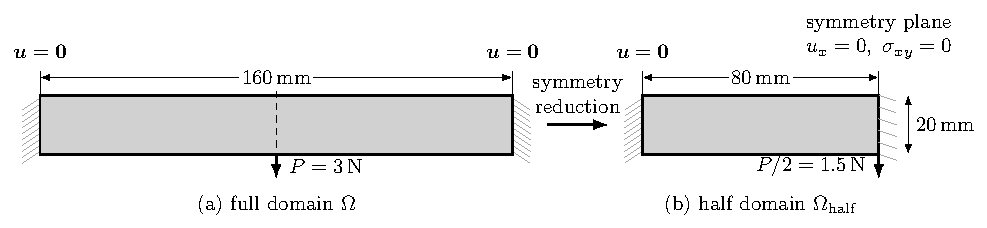
\includegraphics[width=\textwidth]{figures/compliance_beam/fig5_1_schematic}
\caption{Geometry, loading and symmetry boundary conditions of the clamped beam: (a) full design domain; (b) left-half computational domain.}
\label{fig:clamped_beam_schematic}
\end{figure}

Exploiting the symmetry of the geometry and the loading, the computations are carried out on the left half of the domain ($80\,\mathrm{mm}\times20\,\mathrm{mm}$), with the conditions $u_x=0$ and $\sigma_{xy}=0$ on the symmetry plane $x=80\,\mathrm{mm}$. LFEM imposes $u_x=0$ strongly on the horizontal displacement DOFs. In HZMFEM, $u_x=0$ is a natural condition, and $\sigma_{xy}=0$ is imposed strongly by setting the tangential component of the stress normal trace on this edge to zero while leaving the normal component free. The resultant load carried by the half domain is $P/2=1.5\,\mathrm{N}$; in what follows the compliance is reported for the full structure, i.e., twice the value computed on the half domain.

The same uniform right-triangle partition with checkerboard-alternating diagonals as in Section~\ref{subsec:manufactured_solutions} is used with $80\times20$ cells ($N_e=3\,200$ elements on the half domain, equivalent to $6\,400$ elements on the full domain), and the density filter radius is $r_{\min}=2.4\,\mathrm{mm}$. Both discretizations use the MMA update of Algorithm~\ref{alg:compliance_single_loop}, starting from the uniform initial density $\rho_e^{(0)}=\bar{V}$, with move limit $m=0.2$, design-change tolerance $\varepsilon_\rho=10^{-2}$, bounds $0\le\rho_e\le1$, void modulus $E_{\min}=10^{-9}\,\mathrm{MPa}$ and penalization exponent $p_E=3$. LFEM is run with $p=2,3,4$ and HZMFEM with $k=2,3,4$, where $k=2$ uses the jump stabilization and $k=3,4$ the native high-order scheme. The final topologies are compared in Figure~\ref{fig:clamped_beam_topology} (mirrored to the full domain), and the convergence histories are shown in Figure~\ref{fig:clamped_beam_convergence}.

\begin{figure}[htbp]
\centering
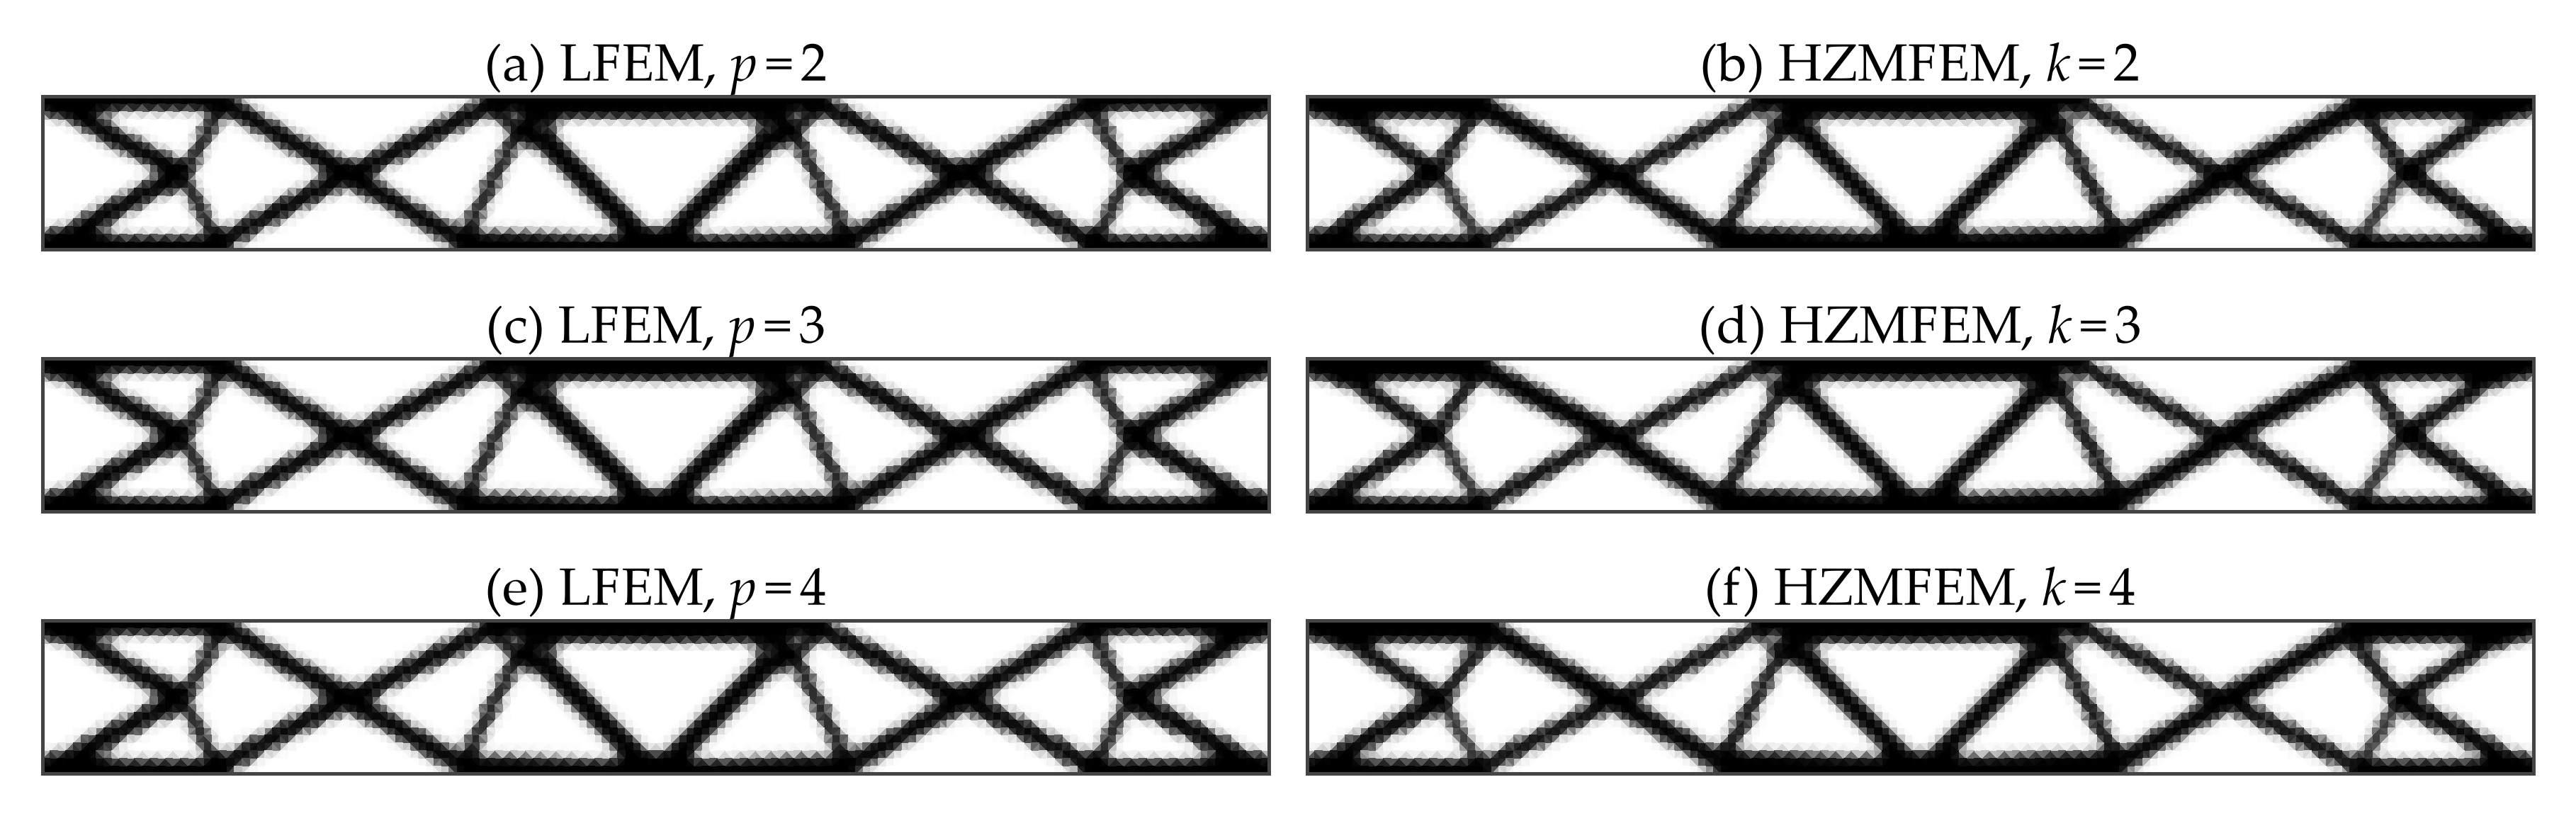
\includegraphics[width=\textwidth]{figures/compliance_beam/compliance_topology}
\caption{Final topologies of the clamped beam obtained with MMA (left column: LFEM, $p$ is the displacement degree; right column: HZMFEM, $k$ is the stress degree).}
\label{fig:clamped_beam_topology}
\end{figure}

\begin{figure}[htbp]
\centering
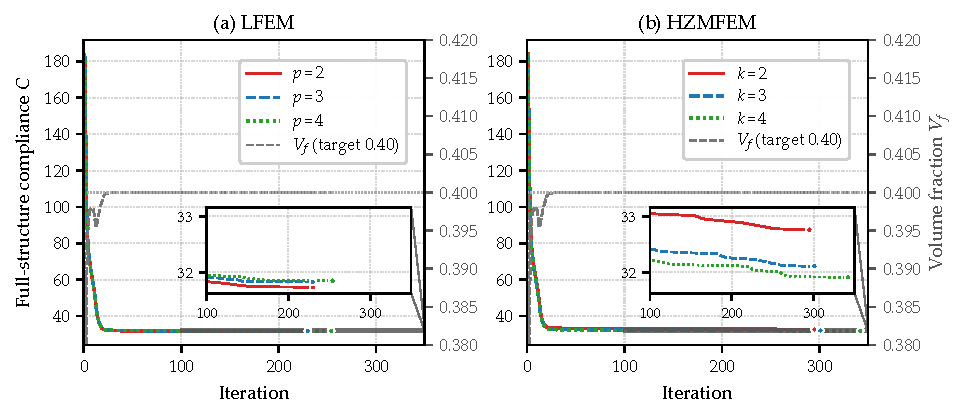
\includegraphics[width=\textwidth]{figures/compliance_beam/compliance_convergence}
\caption{Optimization histories of the clamped beam with MMA (colored curves: full-structure compliance; gray curves: volume fraction; end markers: final compliance of each run, i.e., the optimized compliance in Table~\ref{tab:clamped_beam_reanalysis}; inset: zoom of the late iterations).}
\label{fig:clamped_beam_convergence}
\end{figure}

Figure~\ref{fig:clamped_beam_topology} shows that both methods produce layouts whose main load path consists of crossing diagonal bars, with differences in the connections and thicknesses of individual bars. The three LFEM runs with $p=2,3,4$ reach the design-change tolerance after 230, 230 and 254 iterations, and the three HZMFEM runs with $k=2,3,4$ after 287, 301 and 342 iterations; the final volume fractions are all close to $0.4$ and satisfy the volume constraint (Figure~\ref{fig:clamped_beam_convergence}). The final full-beam compliance of each run evaluated with its own discretization (the optimized compliance) is listed in the third column of Table~\ref{tab:clamped_beam_reanalysis} (in $\mathrm{N\cdot mm}$, likewise below): 31.73, 31.83 and 31.85 for LFEM with $p=2,3,4$, and 32.76, 32.11 and 31.91 for HZMFEM with $k=2,3,4$.

The differences among these optimized compliances cannot be read directly as differences among the final designs. The displacement method evaluates the compliance as the external work and the mixed method as the complementary energy~\eqref{eq:compliance_obj}, so the two give different discrete values even for the same design; moreover, each run solves its own optimization problem independently, and the final designs are not identical. To separate the two factors, the final physical densities of the six runs are frozen, the state equations are solved once with each of LFEM $p=3,4$ and HZMFEM $k=3,4$, and the compliance is evaluated with the corresponding functional; the results are listed in the last four columns of Table~\ref{tab:clamped_beam_reanalysis}.

\begin{table}[htbp]
\centering
\caption{Optimized compliance and uniform reanalysis compliance of the six final designs of the clamped beam (full structure, in $\mathrm{N\cdot mm}$; $p$: displacement degree of LFEM, $k$: stress degree of HZMFEM).}
\label{tab:clamped_beam_reanalysis}
\small
\begin{tabular}{lcccccc}
\toprule
\multirow{2}{*}{Optimized design} & \multirow{2}{*}{Iterations} & Optimized & \multicolumn{4}{c}{Reanalysis compliance} \\
\cmidrule(lr){4-7}
 & & compliance & $p=3$ & $p=4$ & $k=3$ & $k=4$ \\
\midrule
LFEM $p=2$   & 230 & 31.73 & 31.83 & 31.85 & 32.38 & 32.13 \\
LFEM $p=3$   & 230 & 31.83 & 31.83 & 31.85 & 32.38 & 32.13 \\
LFEM $p=4$   & 254 & 31.85 & 31.83 & 31.85 & 32.38 & 32.13 \\
HZMFEM $k=2$ & 287 & 32.76 & 31.60 & 31.63 & 32.13 & 31.88 \\
HZMFEM $k=3$ & 301 & 32.11 & 31.57 & 31.59 & 32.11 & 31.86 \\
HZMFEM $k=4$ & 342 & 31.91 & 31.61 & 31.64 & 32.17 & 31.91 \\
\bottomrule
\end{tabular}
\end{table}

Within each reanalysis column, the compliances of the three LFEM designs differ by at most $0.01\%$ and those of the three HZMFEM designs by at most $0.20\%$, and the maximum relative difference among the six designs is about $0.82\%$ (LFEM columns) and $0.86\%$ (HZMFEM columns), far below the $3.26\%$ spread among the six optimized compliances. On the other hand, for each frozen design the LFEM compliance increases with $p$ while the HZMFEM compliance decreases with $k$, and the relative difference between the two functionals at the same order shrinks from $1.66\%$--$1.78\%$ at order 3 to $0.82\%$--$0.89\%$ at order 4, so the two discrete approximations approach each other from opposite sides. The differences among the optimized compliances therefore stem mainly from the objective functionals and the discretizations rather than from the final designs. This agrees with the observation of Bruggi~\cite{Bruggi2016} that truly mixed and displacement-based elements on regular grids yield almost identical optimal layouts for energy-type TO problems. This example shows that HZMFEM attains load-carrying layouts and final compliances close to those of LFEM in the classical compliance minimization problem, providing numerical support for the correctness of the proposed TO pipeline.

\subsubsection{Nearly Incompressible Topology Optimization (2D Bearing)}
\label{subsubsec:bearing}

The 2D bearing benchmark ($120\,\mathrm{mm}\times40\,\mathrm{mm}$, plane strain, Figure~\ref{fig:bearing_schematic}) is used to examine the resistance to volumetric locking in the nearly incompressible limit. The bottom edge is fully clamped ($u_x=u_y=0$), a uniform downward traction of intensity $t_0=8\times10^{-2}\,\mathrm{N/mm}$ is applied on the top edge, and the left and right edges are traction-free. The material parameters are $E_0=1\,\mathrm{MPa}$, with $\nu_0=0.3$ for the compressible reference group and $\nu_0=0.4999$ for the nearly incompressible group; the void modulus is $E_{\min}=10^{-9}\,\mathrm{MPa}$ and $p_E=3$. The Poisson's ratio is kept fixed in the compressible group, whereas in the nearly incompressible group it is interpolated by~\eqref{eq:poisson_relaxation} with $\nu_{\mathrm{void}}=0.3$ and $p_\nu=1$.

\begin{figure}[htbp]
\centering
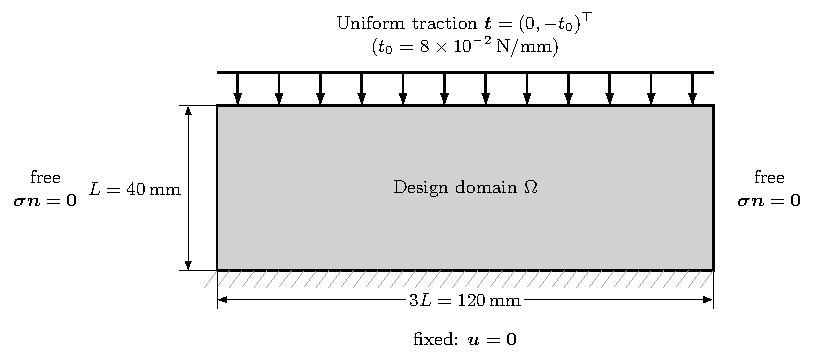
\includegraphics[width=\textwidth]{figures/incompressible/fig5_4_bearing_schematic}
\caption{Geometry and boundary conditions of the 2D bearing.}
\label{fig:bearing_schematic}
\end{figure}

The design domain is discretized by a $120\times40$ structured triangular mesh ($9\,600$ elements) whose diagonals are mirrored between the left and right halves, consistent with the left--right symmetry of the problem. The volume fraction bound is $\bar{V}=0.35$, the density filter radius is $r_{\min}=2.0\,\mathrm{mm}$, and the initial density is uniform, $\rho_e^{(0)}=\bar{V}$. For each material group the problem is solved with LFEM $p=1,2$ and HZMFEM $k=2$ (the latter with the jump stabilization of Section~\ref{subsec:jump_stabilization}), giving six optimization runs in total. All runs use the OC update of Algorithm~\ref{alg:compliance_single_loop} with move limit $m=0.2$, damping exponent $\xi=0.5$ and design-change tolerance $\varepsilon_\rho=10^{-2}$, and all reach the stopping criterion.

Before the optimization, volumetric locking is examined on the fully solid domain ($\rho_e\equiv1$). For $\nu_0=0.3$ and $0.4999$ the mesh is refined from $30\times10$ to $240\times80$; LFEM $p=1,2$ and HZMFEM $k=2$ are computed on four levels, and HZMFEM $k=4$, which needs no stabilization, on the first three. For each Poisson's ratio the reference value is the Richardson-extrapolated limit of the first three HZMFEM $k=4$ results~\cite{Roache1994} (Figure~\ref{fig:bearing_solid_h_convergence}). The limits extrapolated from the other sequences differ from this reference by no more than $0.06\%$, so deviations below this level (the two finest levels of LFEM $p=2$ in the compressible group) are not interpreted quantitatively. On the $120\times40$ mesh, the absolute compliance deviation of LFEM $p=1$ grows from about $0.04\%$ to $16.82\%$ as the Poisson's ratio is increased, a clear sign of locking; those of HZMFEM $k=2$ and $k=4$ grow only from $0.66\%$ and $0.30\%$ to $0.96\%$ and $0.42\%$, and for both Poisson's ratios they decrease monotonically under refinement with similar magnitudes, showing none of the accuracy degradation of the linear displacement element. The deviation of LFEM $p=2$ in the nearly incompressible group is about $0.13\%$, still below that of both mixed discretizations.

\begin{figure}[htbp]
\centering
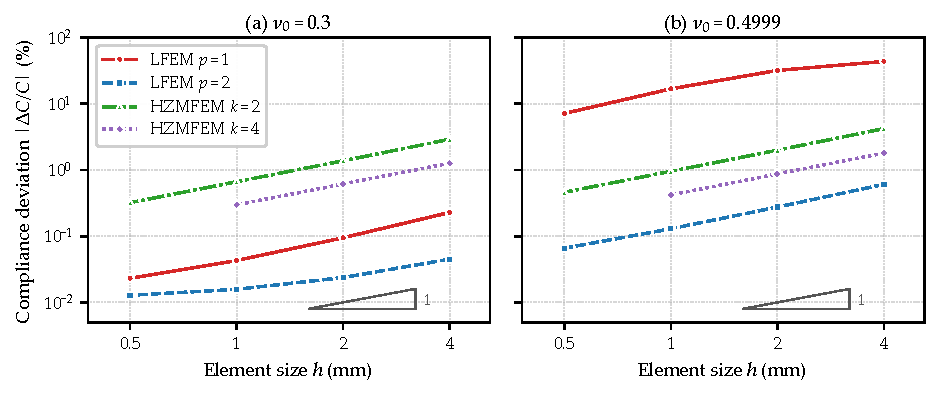
\includegraphics[width=\textwidth]{figures/incompressible/bearing_solid_h_convergence}
\caption{Absolute compliance deviation from the extrapolated reference on the fully solid domain ($\rho_e\equiv1$): (a) $\nu_0=0.3$; (b) $\nu_0=0.4999$.}
\label{fig:bearing_solid_h_convergence}
\end{figure}

Figure~\ref{fig:bearing_topologies} shows the final topologies of the six runs, all of which form a load path dominated by three arches. In the compressible group the three discretizations give similar layouts. In the nearly incompressible group, the arches of LFEM $p=1$ have more polygonal contours with sharper crowns and locally thicker members, whereas LFEM $p=2$ and HZMFEM $k=2$ retain smooth arch contours and give close layouts. Together with the marked accuracy degradation of the linear displacement element in Figure~\ref{fig:bearing_solid_h_convergence}, these differences indicate that volumetric locking has affected its optimization result. In the nearly incompressible group LFEM $p=1$ exhibits a spurious overstiffness due to locking, so its computed compliance is too low (optimized-compliance column of Table~\ref{tab:bearing_reanalysis}) and cannot be taken as evidence of a better design.

\begin{figure}[htbp]
\centering
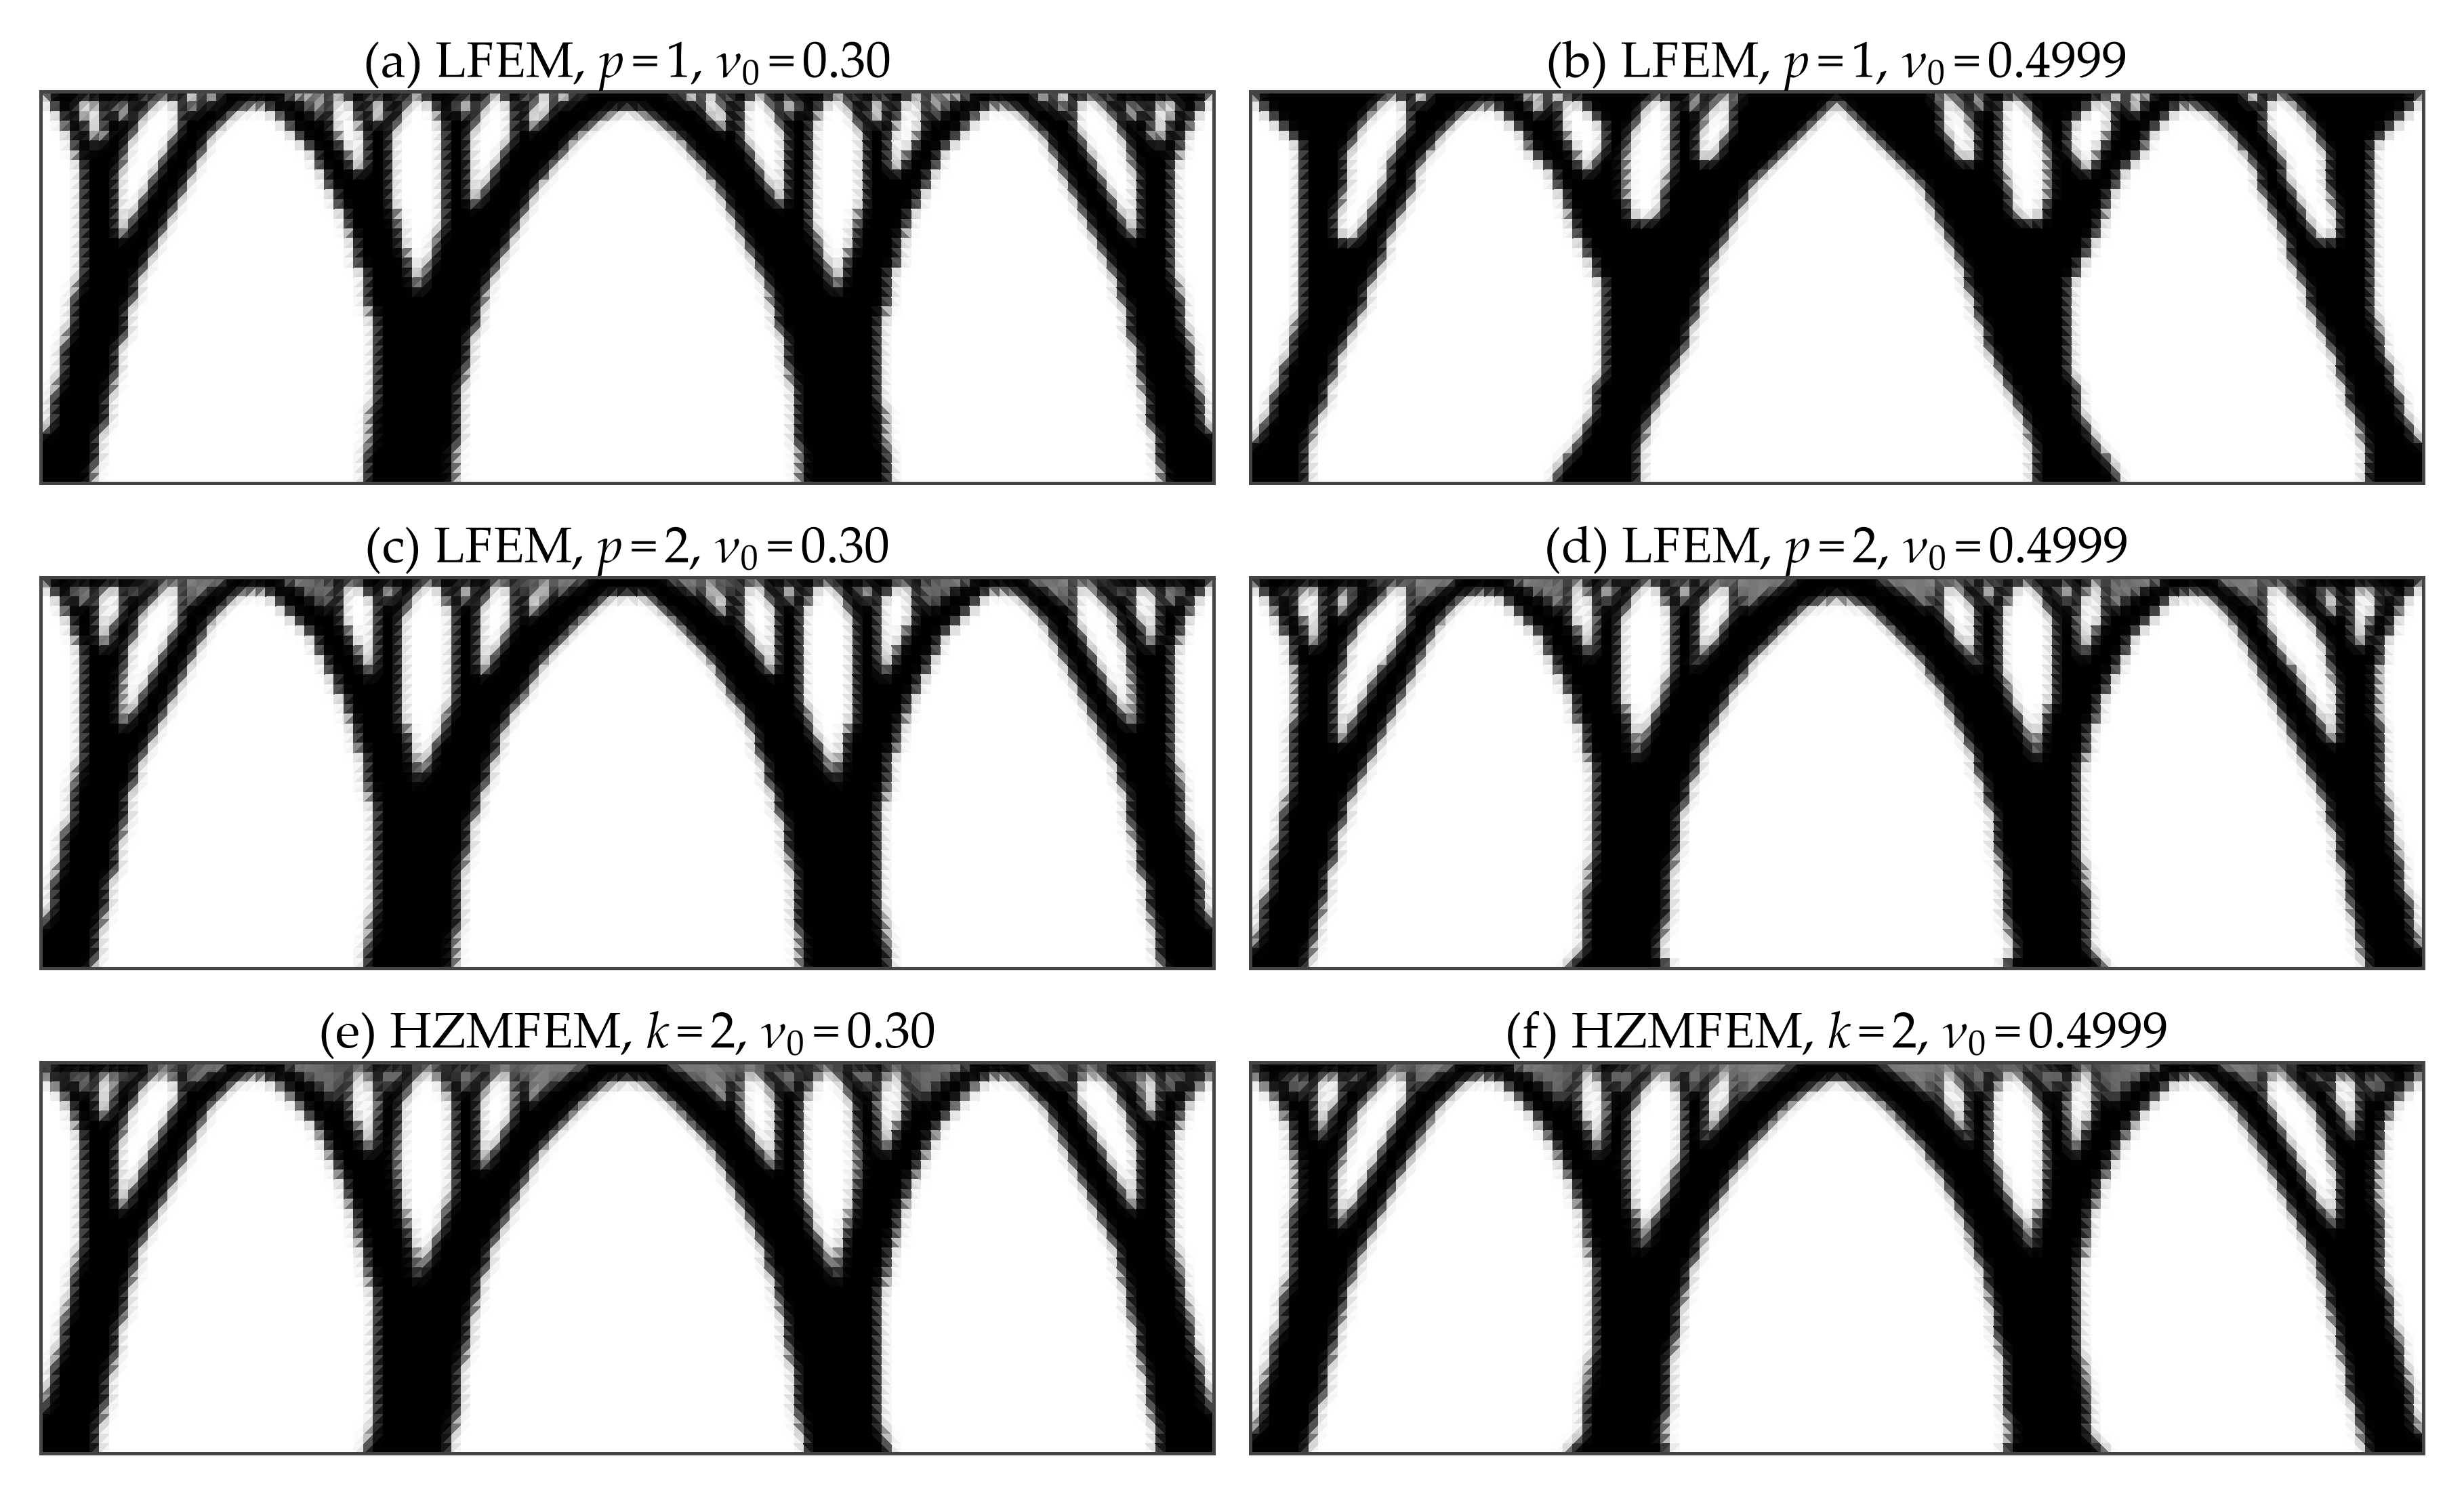
\includegraphics[width=\textwidth]{figures/incompressible/bearing_topologies}
\caption{Final topologies of the 2D bearing (left column: $\nu_0=0.30$; right column: $\nu_0=0.4999$; from top to bottom: LFEM $p=1$, LFEM $p=2$, HZMFEM $k=2$).}
\label{fig:bearing_topologies}
\end{figure}

To compare the six final designs, the physical densities of each run are frozen and reanalyzed on the $120\times40$ mesh with LFEM $p=1,2$ and HZMFEM $k=2,4$; Table~\ref{tab:bearing_reanalysis} lists the HZMFEM $k=4$ compliance together with the relative deviations of the other discretizations from it. Under the common HZMFEM $k=4$ reanalysis, the compliances of the three compressible designs differ by at most about $1.2\%$; in the nearly incompressible group, the design obtained with LFEM $p=1$ has a compliance about $24.0\%$ higher than that obtained with HZMFEM $k=2$, whereas LFEM $p=2$ and HZMFEM $k=2$ differ by only about $0.5\%$. For the same frozen design, the LFEM $p=1$ compliance in the nearly incompressible group is about $17\%$--$38\%$ below the reference value, which further shows that locking overestimates its stiffness. Combining Figures~\ref{fig:bearing_solid_h_convergence} and~\ref{fig:bearing_topologies}, the Hu--Zhang element effectively mitigates the influence of the locking of the linear displacement element on the optimization result, and its designs perform close to those of the quadratic displacement element.

\begin{table}[htbp]
\centering
\caption{Iterations, optimized compliance and HZMFEM $k=4$ reanalysis compliance of the six final designs of the 2D bearing (in $\mathrm{N\cdot mm}$), and relative deviations of the other reanalysis discretizations from the HZMFEM $k=4$ value.}
\label{tab:bearing_reanalysis}
\small
\setlength{\tabcolsep}{4pt}
\begin{tabular}{clcccccc}
\toprule
\multirow{2}{*}{$\nu_0$} & \multirow{2}{*}{Optimized design} & \multirow{2}{*}{Iterations} & Optimized & Reanalysis & \multicolumn{3}{c}{Deviation from $k=4$} \\
\cmidrule(lr){6-8}
 & & & compliance & $k=4$ & $p=1$ & $p=2$ & $k=2$ \\
\midrule
0.30   & LFEM $p=1$   & 281 & 119.33 & 125.83 & $-5.2\%$  & $-1.9\%$ & $+4.9\%$ \\
0.30   & LFEM $p=2$   & 351 & 122.73 & 124.64 & $-4.0\%$  & $-1.5\%$ & $+4.0\%$ \\
0.30   & HZMFEM $k=2$ & 464 & 127.68 & 124.30 & $-3.5\%$  & $-1.2\%$ & $+2.7\%$ \\
\midrule
0.4999 & LFEM $p=1$   & 372 & 76.43  & 123.49 & $-38.1\%$ & $-2.6\%$ & $+4.9\%$ \\
0.4999 & LFEM $p=2$   & 245 & 98.06  & 100.01 & $-17.8\%$ & $-1.9\%$ & $+4.0\%$ \\
0.4999 & HZMFEM $k=2$ & 343 & 102.37 & 99.56  & $-16.8\%$ & $-1.6\%$ & $+2.8\%$ \\
\bottomrule
\end{tabular}
\end{table}

\subsubsection{Local Stress-Constrained Cantilever Beam}
\label{subsubsec:stress_cantilever}

The local stress-constrained cantilever beam (Figure~\ref{fig:cantilever_schematic}) has a design domain of $80\,\mathrm{mm}\times40\,\mathrm{mm}$ in plane stress, clamped along the left edge. A vertical resultant $P=400\,\mathrm{N}$ at the midpoint of the right edge is applied as a uniform traction $\bar t=P/l$ over a contact width $l=6\,\mathrm{mm}$ whose end points coincide with mesh nodes. The displacement method imposes this load through the boundary integral and the mixed method through the normal trace of the stress; the neighborhoods of the contact end points are treated as passive solid regions as described below. The solid material is an aluminum alloy with $E_0=70\,000\,\mathrm{MPa}$, $\nu_0=0.25$ and allowable stress $\bar\sigma=180\,\mathrm{MPa}$, and the void modulus is $E_{\min}=10^{-9}E_0$. Since the load is design-independent and the displacement boundary conditions are homogeneous, the stresses do not depend on the scale of the elastic moduli; the computations therefore use $E_0^{\mathrm{calc}}=1\,\mathrm{MPa}$, with $E_{\min}$ and the stabilization coefficient of the stabilized $k=2$ scheme used later in this section scaled proportionally, while the load and $\bar\sigma$ keep their physical values. The penalization exponent is $p_E=3.5$, the domain is discretized by an $80\times40$ checkerboard triangular mesh with alternating diagonals ($6\,400$ elements), the density filter radius is $r_{\min}=6.0\,\mathrm{mm}$, and the initial density is $\rho_e^{(0)}=0.5$.

\begin{figure}[htbp]
\centering
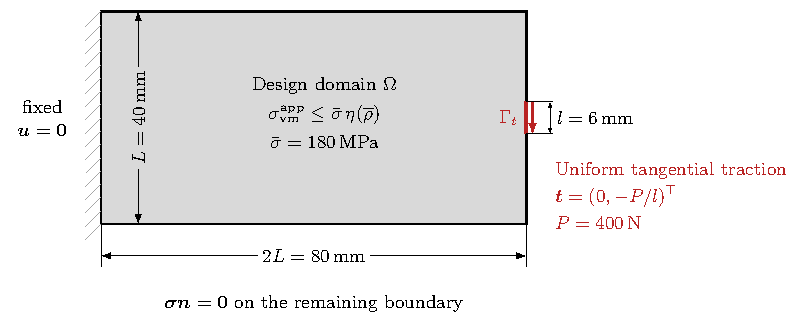
\includegraphics[width=\textwidth]{figures/stress_constrained/fig5_6_cantilever_schematic}
\caption{Design domain, local load and boundary conditions of the 2D cantilever beam.}
\label{fig:cantilever_schematic}
\end{figure}

Both methods use the same mesh, load and optimization parameters. LFEM uses $p=3$ and HZMFEM uses $k=3$, the latter being a native high-order scheme that needs no jump stabilization. The filtered density is passed through the tanh projection~\eqref{eq:heaviside_projection} with $\eta_{\mathrm p}=0.5$, and $\beta$ is increased from $1$ by $1$ every 5 outer iterations up to $10$. The local stress constraints follow the model of Section~\ref{subsec:stress_constraints} with $\epsilon=10^{-3}$ held fixed throughout. A passive solid region $\Omega_{\mathrm{pad}}$ is defined as the neighborhoods of radius $r_{\mathrm{pad}}=1.5\,\mathrm{mm}$ around the two end points of the contact width (16 elements for both discretizations, $0.25\%$ of the design domain area). No local stress constraint is imposed there, i.e. the region is left out of the stress-constraint term of the augmented Lagrangian, as for the elements around concentrated loads in Bruggi and Venini~\cite{BruggiVenini2008}. Its physical density is set to $1$ after filtering and projection and the corresponding derivative of the density mapping is set to zero, so that the region is excluded from the optimization as in Holmberg et al.~\cite{Holmberg2013}. Its volume is counted in the total volume fraction. The criterion set is $\mathcal E_{\mathrm{acc}}=\{e\notin\Omega_{\mathrm{pad}}:\bar\rho_e\geq0.5\}$; the elements with $\bar\rho_e<0.5$ still carry the relaxed stress constraint but do not enter the stopping test. The ALM--MMA procedure of Algorithm~\ref{alg:stress_alm_mma} is used with $\mu_0=50$, $\gamma_\mu=1.1$, $\mu_{\max}=10^4$, $\lambda_{\max}=3000$, move limit $m=0.15$, a minimum asymptote gap of $10^{-4}$, $N_{\mathrm{out}}^{\max}=200$ and $N_{\mathrm{in}}^{\max}=5$. The stopping parameters are $\delta_\rho=0.002$, $\delta_g=0.005$ and $N_{\mathrm{hold}}=3$.

\begin{figure}[htbp]
\centering
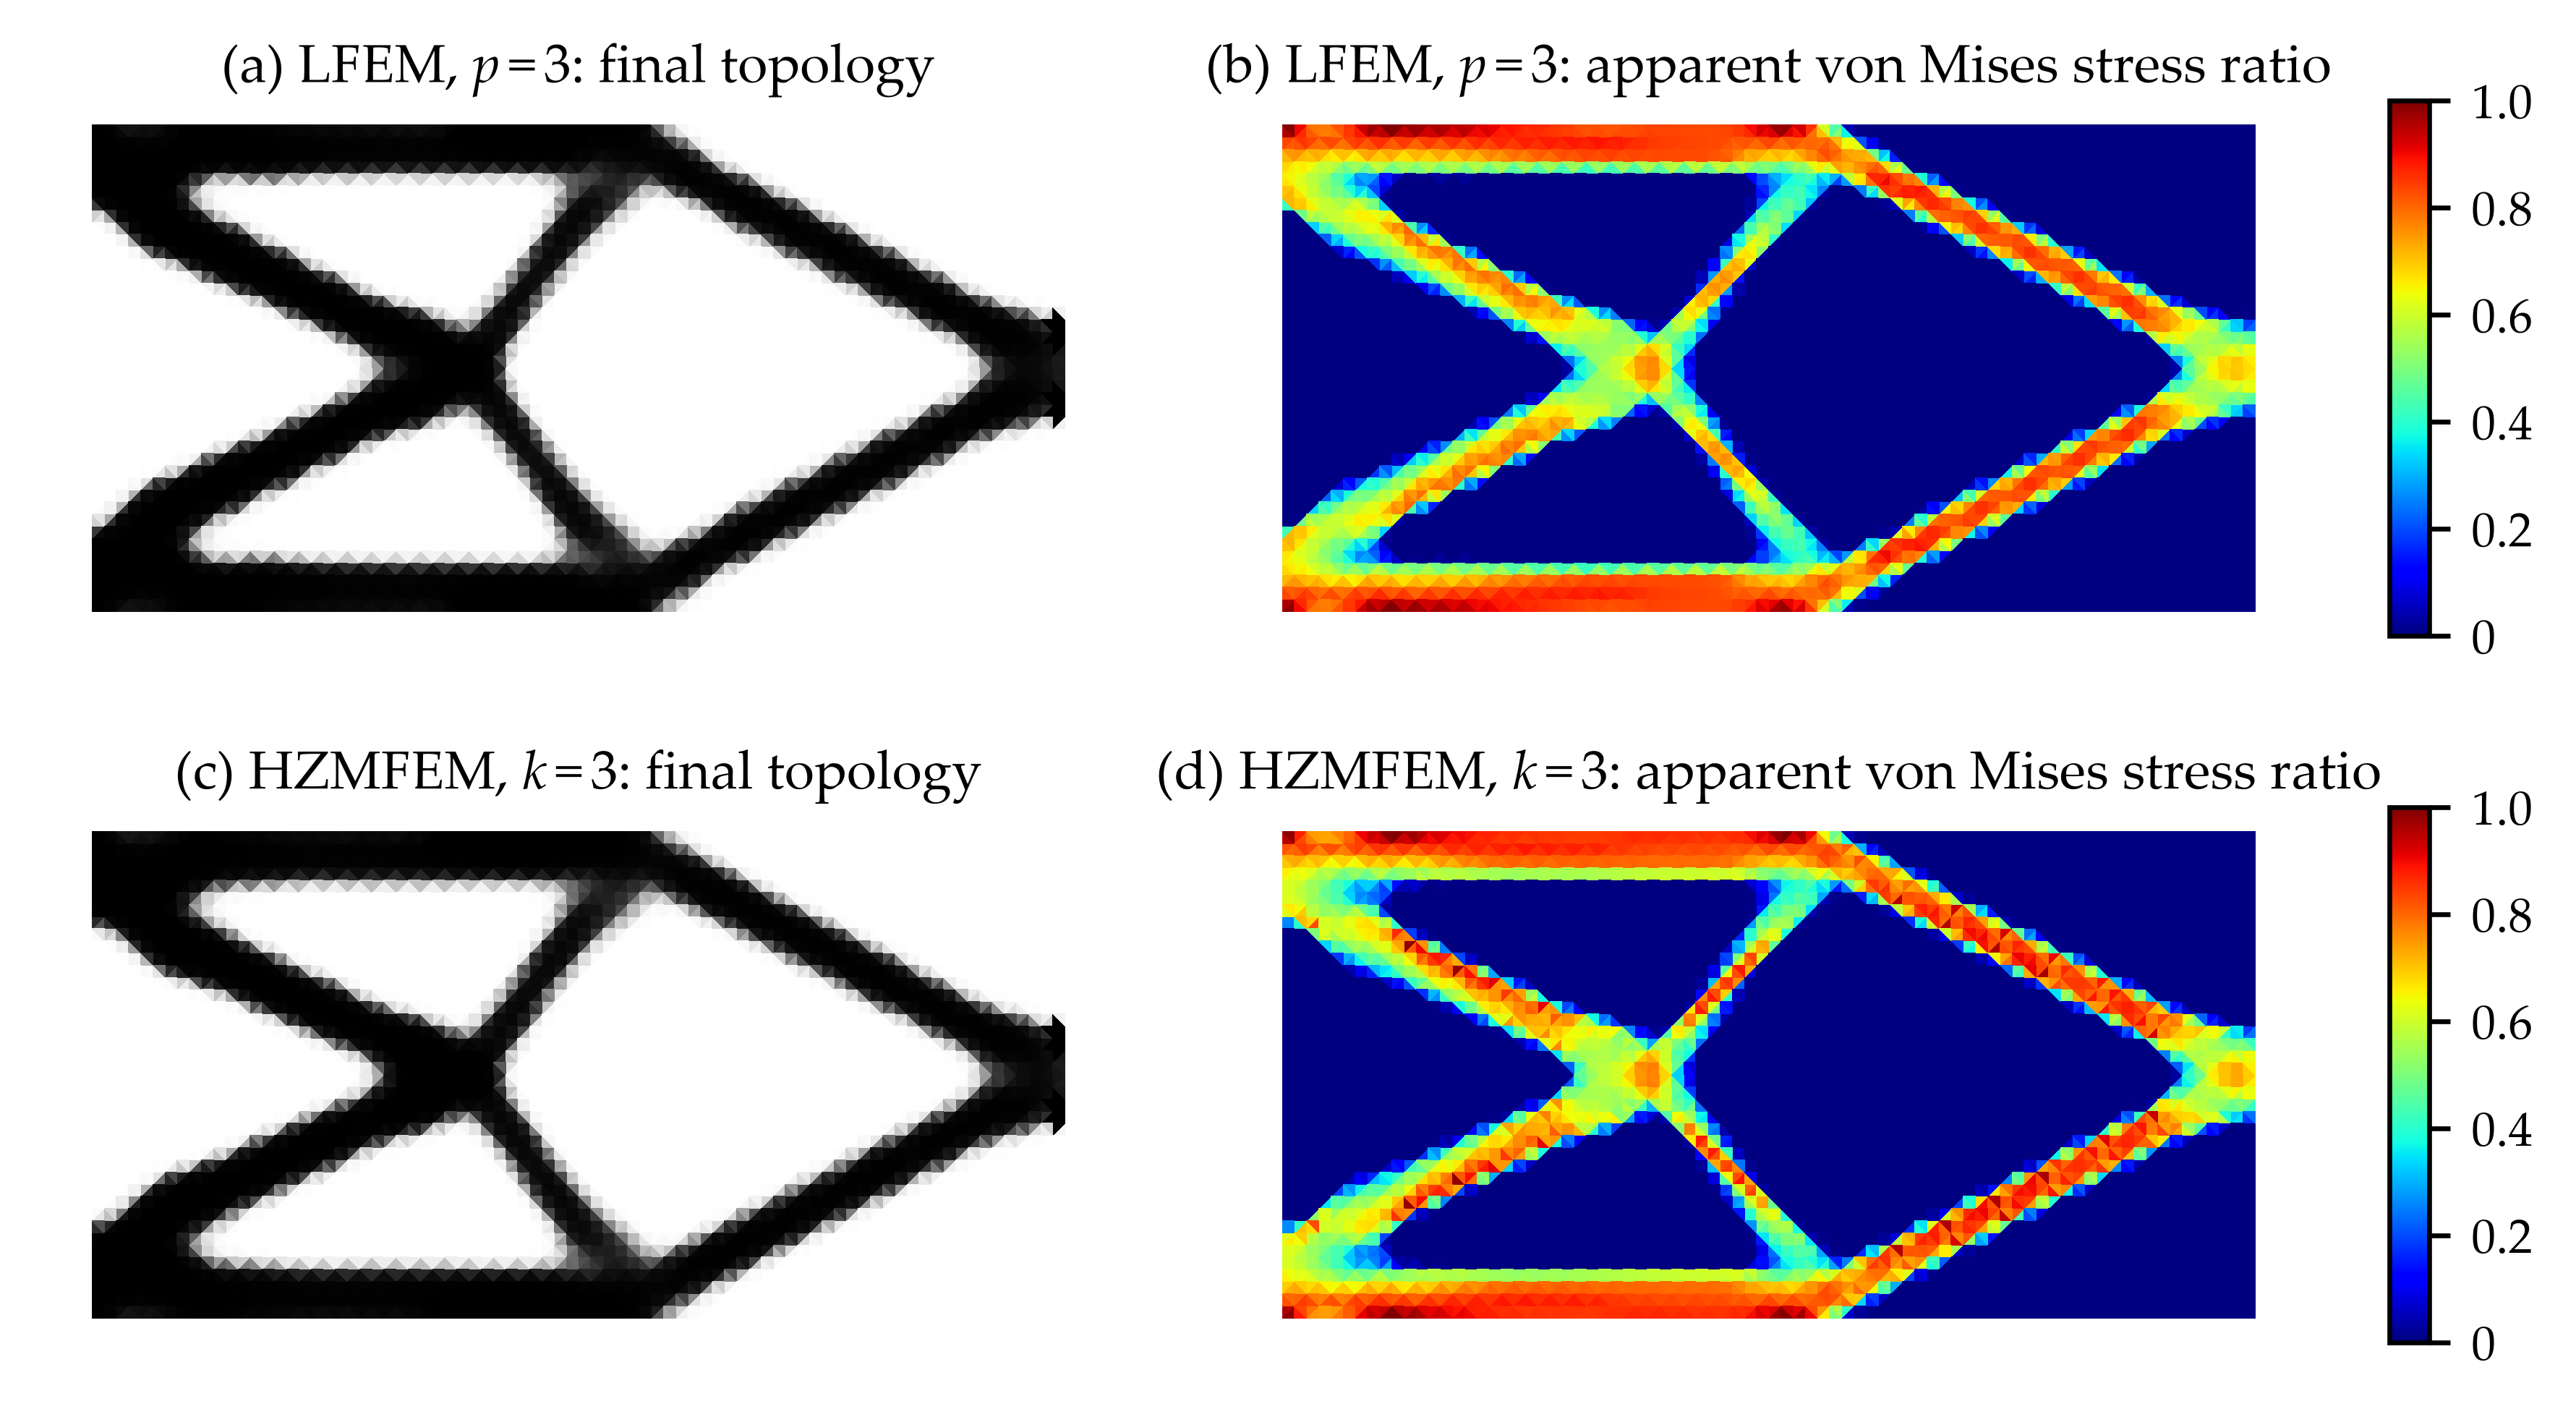
\includegraphics[width=\textwidth]{figures/stress_constrained/stress_cubic_topologies}
\caption{Final topologies and apparent von Mises stress ratio of the cantilever beam with cubic discretizations (LFEM: $p=3$; HZMFEM: $k=3$).}
\label{fig:stress_cubic_topologies}
\end{figure}

Figure~\ref{fig:stress_cubic_topologies} shows that the two discretizations give similar truss-like topologies: the main load path consists of the upper and lower chords and the internal crossing diagonals, the high-stress regions are distributed along this path, and both the layout and the stress distribution are close between the two discretizations.

\begin{figure}[htbp]
\centering
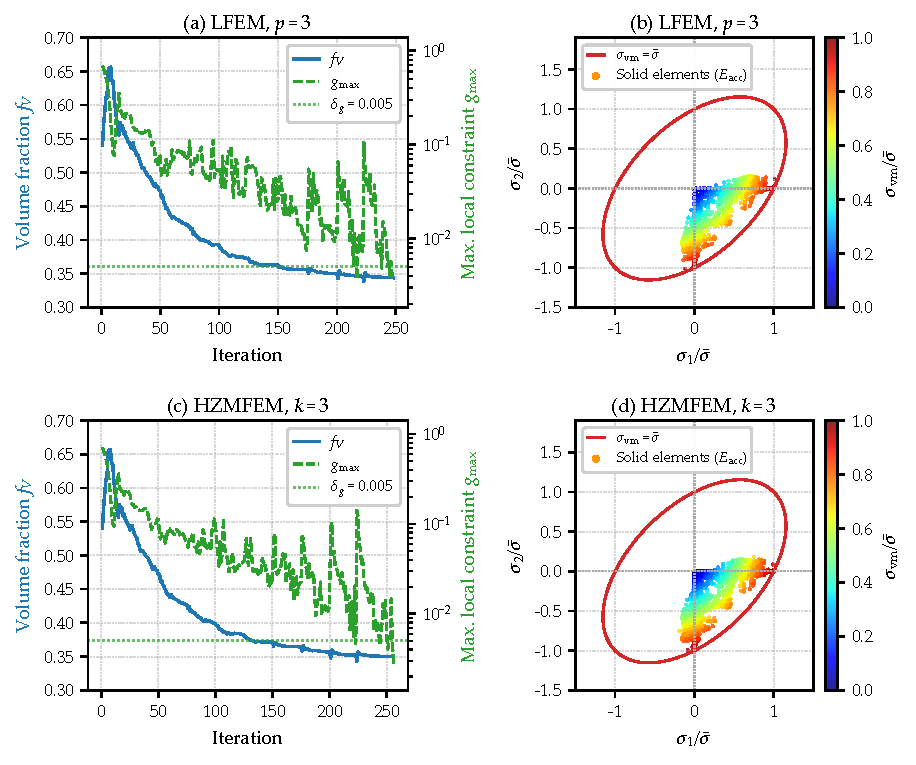
\includegraphics[width=\textwidth]{figures/stress_constrained/stress_cubic_convergence}
\caption{Convergence histories and element stress distributions in the principal stress plane for the cantilever beam with cubic discretizations ((a,b) LFEM $p=3$; (c,d) HZMFEM $k=3$); $g_{\max}$ and the stress points are evaluated on the criterion set $\mathcal E_{\mathrm{acc}}$.}
\label{fig:stress_cubic_convergence}
\end{figure}

Figure~\ref{fig:stress_cubic_convergence}(a,c) shows the histories of the volume fraction and of the maximum local constraint value on the criterion set $\mathcal E_{\mathrm{acc}}$, each constraint being evaluated with its own discretization. LFEM and HZMFEM reach the stopping criterion of Algorithm~\ref{alg:stress_alm_mma} after 248 and 256 MMA updates, respectively; the final $f_V$ are $34.39\%$ and $35.01\%$, and the final $g_{\max}$ are $3.92\times10^{-3}$ and $2.82\times10^{-3}$, both below $\delta_g=0.005$. Figure~\ref{fig:stress_cubic_convergence}(b,d) shows the ratios $\sigma_i/\bar\sigma$ ($\sigma_1\geq\sigma_2$) of the apparent principal stresses at the element centroids to the allowable stress for the elements in $\mathcal E_{\mathrm{acc}}$, colored by the apparent von Mises stress ratio. The stress points lie almost entirely in the quadrant $\sigma_1\geq0\geq\sigma_2$: part of them cluster along the two axes, i.e. in uniaxial tension or compression, in line with the axial load-carrying of the members of the truss-like layout, while the rest spread between the axes up to the yield ellipse, i.e. in biaxial tension--compression states dominated by shear.

With the same settings as in Figure~\ref{fig:stress_cubic_topologies}, the problem is also solved with the stabilized scheme $k=2$ and the native scheme $k=4$; the results are shown in Figure~\ref{fig:stress_hz_orders_topologies}. Together with $k=3$, the three orders take 250, 256 and 258 MMA updates, the final $f_V$ are $34.70\%$, $35.01\%$ and $35.30\%$, and the final $g_{\max}$ on the criterion set $\mathcal E_{\mathrm{acc}}$ are $1.96\times10^{-3}$, $2.82\times10^{-3}$ and $4.92\times10^{-3}$, all below $\delta_g$ and all satisfying the same design-change criterion. The three orders give similar main load-carrying layouts, showing that the optimization procedure applies to both the low-order stabilized and the high-order native discretizations considered.

\begin{figure}[htbp]
\centering
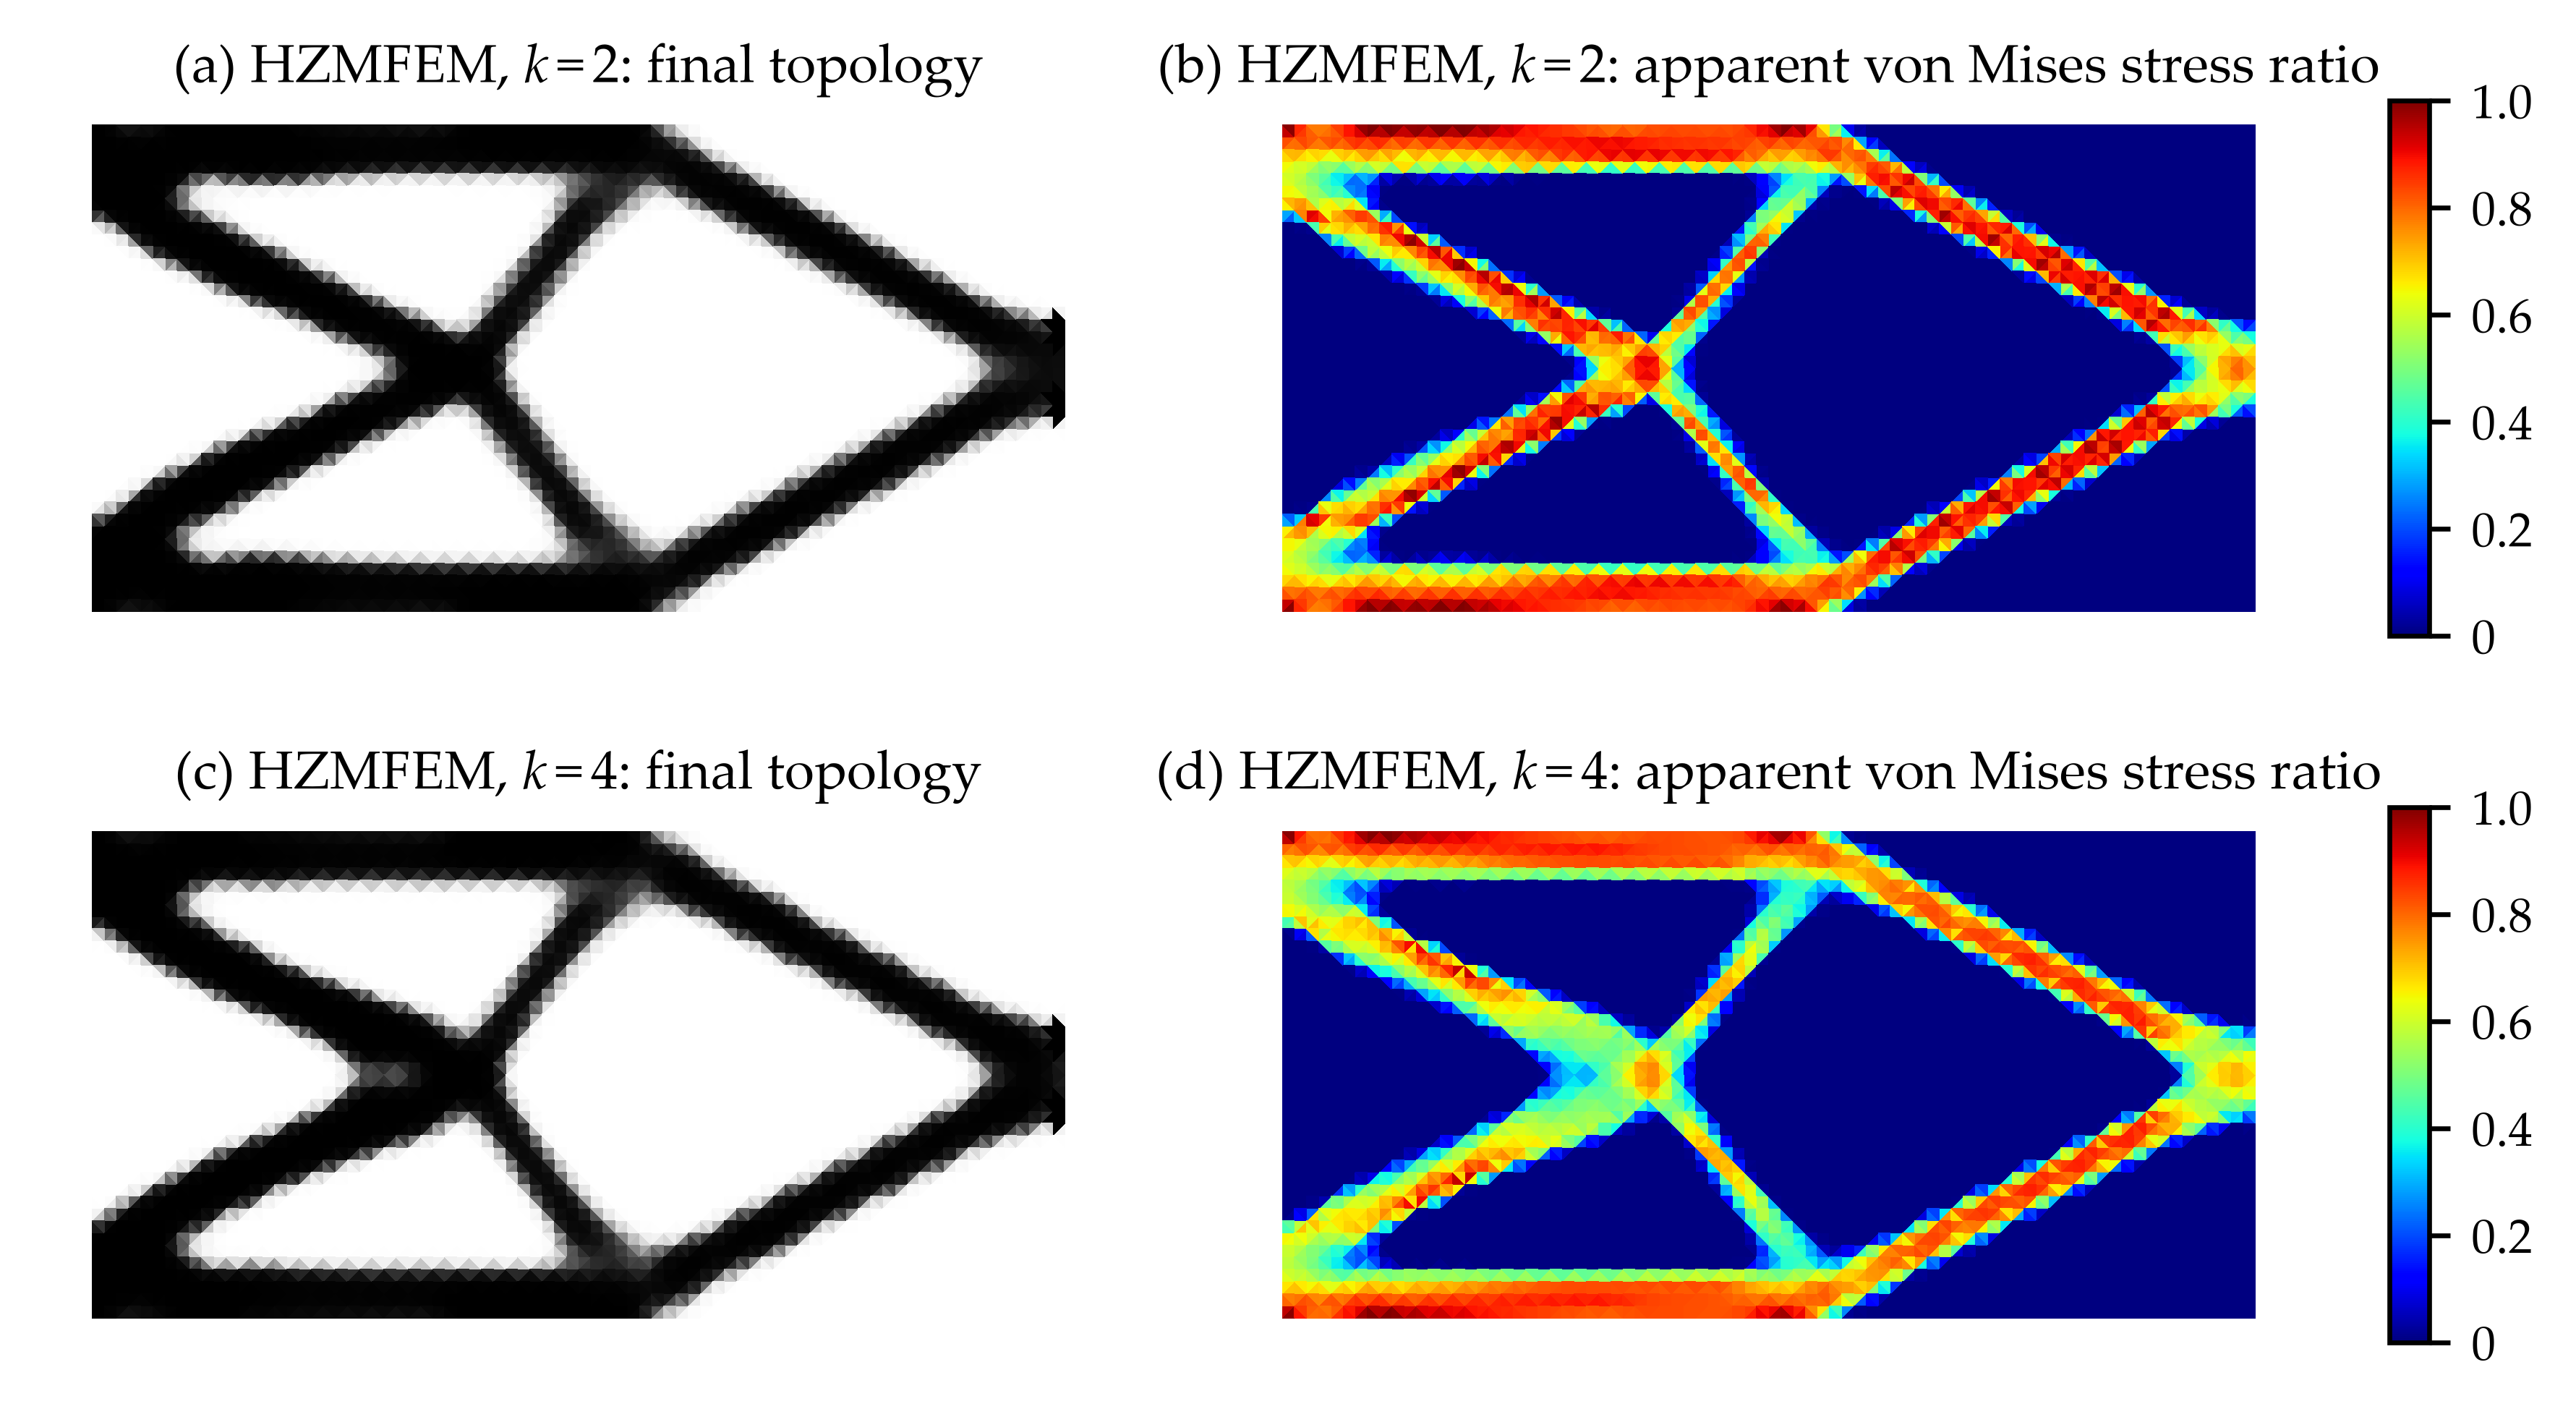
\includegraphics[width=\textwidth]{figures/stress_constrained/stress_hz_orders_topologies}
\caption{Final topologies and apparent von Mises stress ratio of the cantilever beam with Hu--Zhang mixed discretizations ((a,b) $k=2$; (c,d) $k=4$).}
\label{fig:stress_hz_orders_topologies}
\end{figure}

To examine the stress fields of the two discretizations further, we compare their inter-element normal traction continuity. For HZMFEM, $g_e$ is taken directly from the primary unknown $\boldsymbol{\sigma}_h\in H(\operatorname{div},\Omega;\mathbb S)$, whose normal traction is single-valued across elements; for LFEM, the stress is recovered element by element from the displacement gradient, and the traction is discontinuous on interior faces. To quantify this difference, the six final designs of LFEM $p=2,3,4$ and HZMFEM $k=2,3,4$ (those for $p=2,4$ are obtained separately with the settings and stopping criterion of Figure~\ref{fig:stress_cubic_topologies}) are re-solved for the state equations with the discretization used in their optimization. On an interior face $F$ we define the normalized root-mean-square traction jump $A_F$, and take the maximum over the interior faces of an element as the element indicator $A_e$:
\begin{equation}
\label{eq:traction_jump_indicator}
A_F=\frac{1}{\bar\sigma}\Big(\frac{1}{|F|}\int_F\big\|\llbracket\boldsymbol{\sigma}^{\mathrm{app}}_h\boldsymbol{n}\rrbracket\big\|^2\,\mathrm{d}s\Big)^{1/2},\qquad A_e=\max_{F\subset\partial T_e\cap\Omega}A_F.
\end{equation}
The statistics are restricted to the solid band ($\bar\rho_e>0.9$ and $e\notin\Omega_{\mathrm{pad}}$). In Figure~\ref{fig:stress_traction_jump}, $A_e$ of the three HZMFEM orders is at round-off level (at most $2.2\times10^{-16}$); for LFEM $p=2,3,4$ the medians of $A_e$ are $2.4\times10^{-2}$, $1.6\times10^{-2}$ and $1.1\times10^{-2}$ and the 95th percentiles are $0.13$, $0.086$ and $0.072$, decreasing with the order but remaining clearly non-zero, with the larger jumps concentrated at the member edges. This reflects the difference between the two discretizations in inter-element equilibrium: the Hu--Zhang stress field preserves normal traction continuity, whereas a stress recovered element by element from the displacement gradient does not satisfy this continuity in general. The lines $\delta_g$ and $4\delta_g$ in the figure serve only as numerical scale references and are not acceptance thresholds for the traction jump.

\begin{figure}[htbp]
\centering
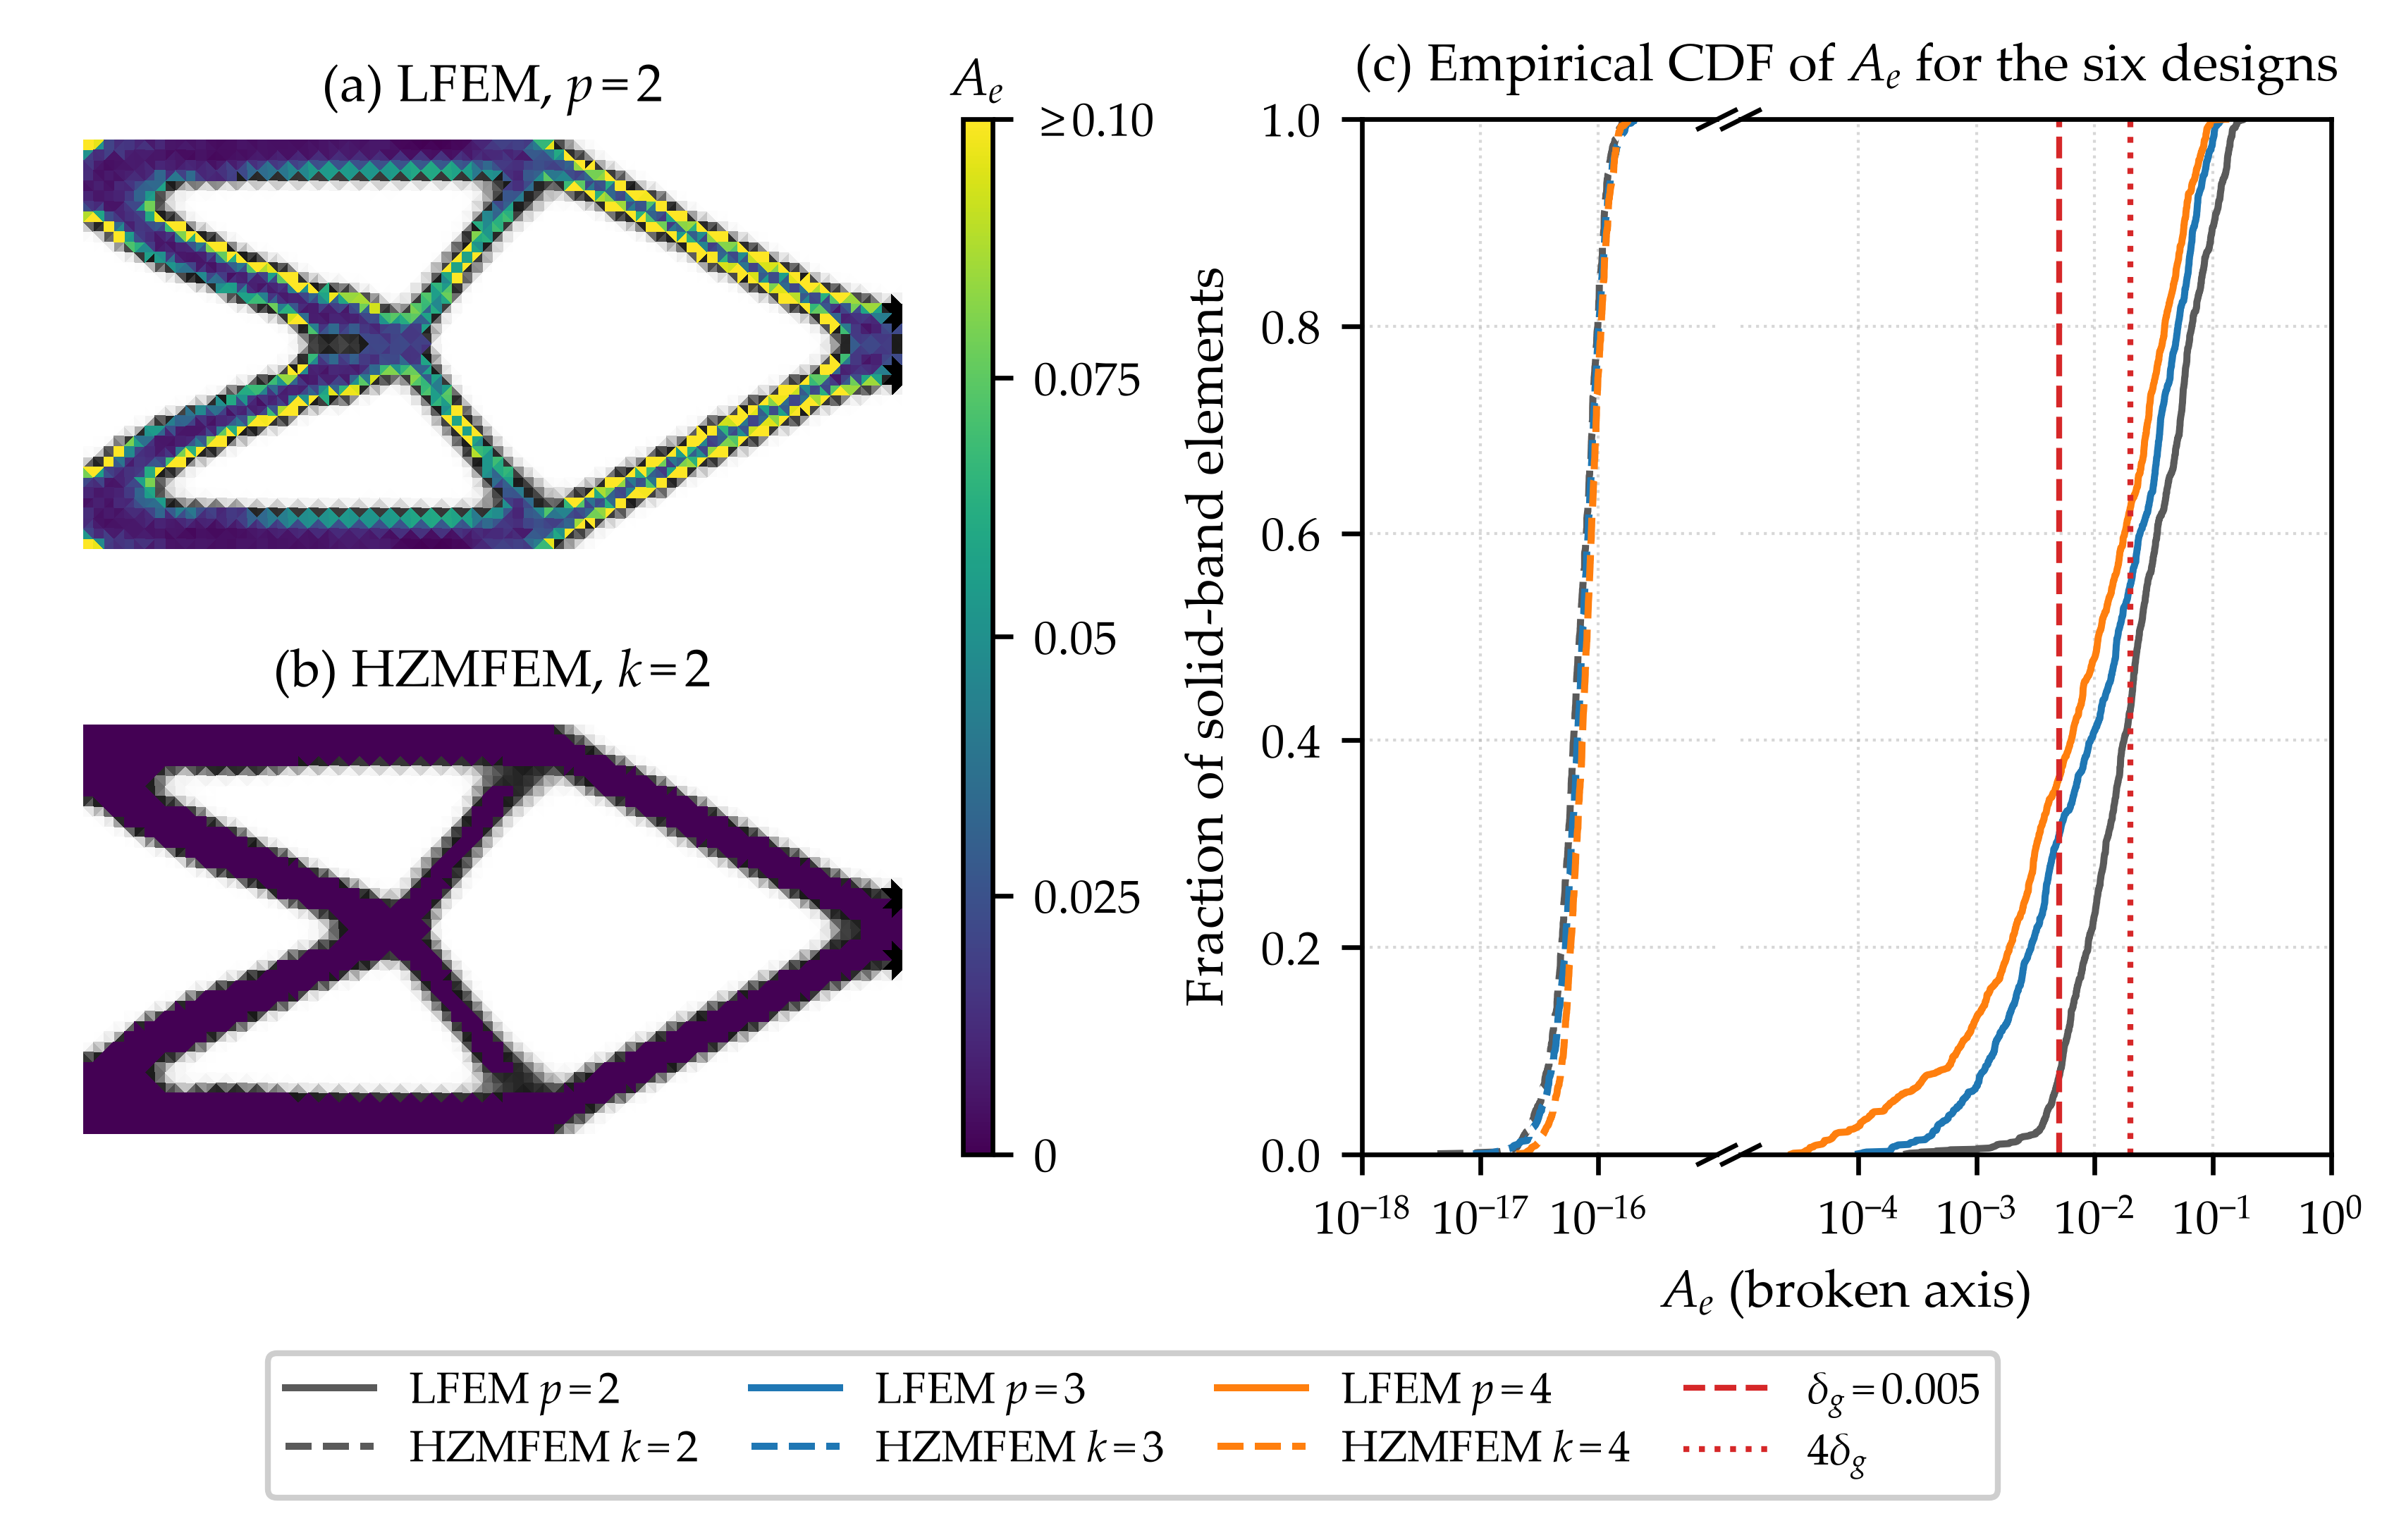
\includegraphics[width=\textwidth]{figures/stress_constrained/stress_traction_jump}
\caption{Element-wise traction jump $A_e$ on the solid band of the final designs: spatial distribution for (a) LFEM $p=2$ and (b) HZMFEM $k=2$ (shared color scale, values above the upper bound are clipped); (c) empirical cumulative distributions of the six designs on a broken horizontal axis, the left part for HZMFEM $k=2$--$4$ (dashed) and the right part for LFEM $p=2$--$4$ (solid), with vertical lines at $\delta_g$ and $4\delta_g$.}
\label{fig:stress_traction_jump}
\end{figure}

\section{Concluding Remarks}
\label{sec:conclusions}

\subsection{Key Conclusions}
\label{subsec:key_conclusions}

In this paper, we have systematically established an arbitrary-order Hu--Zhang mixed finite element framework for density-based continuum topology optimization on simplicial meshes. By adopting the Hellinger--Reissner variational principle with independent symmetric Cauchy stress and displacement fields, the proposed methodology overcomes the primary bottlenecks of classical displacement-based models. The main conclusions are:
\begin{enumerate}
    \item \textbf{Exact Normal Traction Continuity and Stress Fidelity}: The trial stress field naturally resides in $H(\operatorname{div},\Omega;\mathbb{S})$, guaranteeing inter-element normal traction continuity. This fundamentally avoids the stress degradation and inter-element jumps inherent in displacement post-processing, providing an accurate foundation for local stress constraints.
    \item \textbf{Locking-Free Nearly Incompressible Design}: Because the compliance bilinear form remains uniformly bounded as $\nu \to 0.5$, the mixed formulation completely eliminates volumetric locking on general simplicial meshes, without requiring specialized selective integration or artificial pressure projections.
    \item \textbf{Consistent Lifting and Adjoint Formulations}: By introducing design-independent traction lifting, non-homogeneous Neumann boundary conditions are seamlessly resolved, with the design-dependence of the resulting right-hand side rigorously accounted for in the adjoint sensitivity analysis.
\end{enumerate}

\subsection{Future Work and Outlook}
\label{subsec:future_work}

Future research directions include:
\begin{enumerate}
    \item Extending the arbitrary-order mixed topology optimization framework to full three-dimensional tetrahedral meshes;
    \item Developing adaptive mesh refinement (AMR) and $hp$-adaptive strategies driven by Hu--Zhang mixed residual-based error estimators;
    \item Integrating geometric nonlinearity and elastoplastic constitutive laws into the mixed topology optimization formulation.
\end{enumerate}


\section*{Acknowledgments}

\bibliographystyle{abbrv}
\bibliography{references}

\end{document}
